% WSCG sample document 
%
% based on Gabriel Zachmann's sample
% http://zach.in.tu-clausthal.de/latex/
%
% modified Apr 2012 to match WSCG Word template
%
\documentclass[twoside,twocolumn,10pt]{article}
%\documentclass[twoside,twocolumn,draft]{article}

%  for debugging
%\tracingall%\tracingonline=0
%\tracingparagraphs
%\tracingpages

\usepackage{biblatex}
\usepackage[utf8]{inputenc}
\usepackage{amsmath}
\addbibresource{references.bib}

\usepackage{subfig}




%%%%%%%%%%%%%%%%%%%%%%%%%%%%%%%%%%%%%%%%%%%%%%%%%%%%%%%%%%%%%%%%%%%%%%%%%%%%%
%                             Packages

\usepackage{wscg}           % includes a number of other packages (e.g., myalgorithm)
\RequirePackage{ifpdf}
\ifpdf
 \RequirePackage[pdftex]{graphicx}
 \RequirePackage[pdftex]{color}
 
\else
 \RequirePackage[dvips,draft]{graphicx}
 \RequirePackage[dvips]{color}
\fi
%\usepackage[german,english]{babel}     % default = english
%\usepackage{mypicture}      % loads graphicx.sty, color.sty, eepic.sty
%\usepackage{array}          % better tabular's & arrays, plus math tabular's
%\usepackage{tabularx}      % for selfadjusting p-columns
%\setlength{\extrarowheight}{1ex}   % additional space between rows
%\usepackage{booktabs}      % typographically much better
%\usepackage{mdwlist}        % for compacted lists, and more versatile lists
%\usepackage[intlimits]{amsmath} % more math stuff, see texdoc amsldoc
%\usepackage{mymath}         % own commands, loads amssymb & array.sty
%\usepackage{hyphenat}      % hyphenatable -, /, etc.
%\usepackage{theorem}
%\usepackage[sort&compress]{natbib}% better \cite commands, more flexible
%\usepackage[sort&compress,super]{natbib} % better \cite commands, more flexible
%\newcommand{\citenumfont}[1]{\textit{#1}}


\usepackage{nopageno}       % no page numbers at all; uncomment for final version
\usepackage{bm} 
\usepackage{amsmath,amsfonts,amssymb}

\usepackage{todonotes}

%%%%%%%%%%%%%%%%%%%%%%%%%%%%%%%%%%%%%%%%%%%%%%%%%%%%%%%%%%%%%%%%%%%%%%%%%%%%%
%                                Title


\title{Fast triangle-based glyph rendering for high angular resolution diffusion imaging on multimodal visualization environment}

\author{
\parbox{0.25\textwidth}{\centering
Daniel Silva\\[1mm]
DCA/FEEC/University of Campinas,\\
%1st line of address\\
%2nd line of address\\
Brazil\\[1mm]
danielxs@dca.fee.unicamp.br
}
\hspace{0.05\textwidth}
\parbox{0.25\textwidth}{\centering
Second Author\\[1mm]
author's affiliation\\
1st line of address\\
2nd line of address\\
Country (ZIP) code, City, State\\[1mm]
e@mail
}
\hspace{0.05\textwidth}
\parbox{0.25\textwidth}{\centering
Third Author\\[1mm]
author's affiliation\\
1st line of address\\
2nd line of address\\
Country (ZIP) code, City, State\\[1mm]
e@mail
}
}

%%%%%%%%%%%%%%%%%%%%%%%%%%%%%%%%%%%%%%%%%%%%%%%%%%%%%%%%%%%%%%%%%%%%%%%%%%%%%
%                          Hyperref


% no hyperlinks
\usepackage{url}
\urlstyle{tt}

% Donald Arsenau's fix for missing kerning of "//" and ":/"
\makeatletter
\def\Uslash{\mathbin{\mathchar`\/}\@ifnextchar{/}{\kern-.15em}{}}
\g@addto@macro\UrlSpecials{\do \/ {\Uslash}}
\def\Ucolon{\mathbin{\mathchar`:}\@ifnextchar{/}{\kern-.1em}{}}
\g@addto@macro\UrlSpecials{\do : {\Ucolon}}
\makeatother

%added by Ting
\usepackage[normalem]{ulem}
\usepackage{todonotes}

%%%%%%%%%%%%%%%%%%%%%%%%%%%%%%%%%%%%%%%%%%%%%%%%%%%%%%%%%%%%%%%%%%%%%%%%%%%%%
%                              My Commands


%\DeclareMathOperator{\sgn}{sgn}

%\theorembodyfont{\upshape}
%\theoremstyle{break}
%\theoremheaderfont{\bfseries\normalsize}

%\newtheorem{lem}{Lemma}
%\newtheorem{defn}{Definition}

%%%%%%%%%%%%%%%%%%%%%%%%%%%%%%%%%%%%%%%%%%%%%%%%%%%%%%%%%%%%%%%%%%%%%%%%%%%%%
%                                Document


\begin{document}

\twocolumn[{\csname @twocolumnfalse\endcsname

\maketitle  % full width title


\begin{abstract}
\noindent

Diffusion magnetic resonance imaging provides the quantification of the diffusion process of water molecules. Applied to the brain, it is unique in providing white matter fiber structures and connectivity in-vivo, relying on the fact that the water molecules' displacements are greater along with the fiber orientation than perpendicular to it due to biological barriers. For reconstructing multiple fibers passing through the same voxel, high angular resolution diffusion imaging (HARDI) acquisition scheme has been introduced. Advanced methods for processing diffusion data were developed to synthesize HARDI data into orientation distribution functions (ODF), consisting in an association between directions and probabilities of water diffusion along with these directions on the sphere. Visualizing ODFs helps in gaining insight into the local structure of the brain white matter. In this work, we present an interactive GPU triangle-based rendering scheme for ODF. We show how the advanced GPU features may be exploited to make the triangle-based rendering competitive with the ray-casting one, despite ODF data's high dimensionality. Performance measurements are presented to demonstrate the proposed GPU-based rendering algorithm's interactivity.


%We describe the formatting guidelines for the Journal of WSCG and WSCG proceedings adapted from the ACM and SIGGRAPH proceedings and recent WSCG templates.  Please, try to fix format of your contribution as close as possible if you use other tools.

\end{abstract}

\subsection*{Keywords}
%Keywords are your own designated keywords - Times New Roman, 10pts.
medical imaging, HARDI, computer graphics, visualization. 

\vspace*{1.0\baselineskip}
}]

\todo[inline]{Is ODF a representation of HARDI data or a representation of a HARDI data processing tool?}

\todo[inline]{In our approach ... you should }

%%%%%%%%%%%%%%%%%%%%%%%%%%%%%%%%%%%%%%%%%%%%%%%%%%%%%%%%%%%%%%%%%%%%%%%%%%%%%
\section{Introduction}

\copyrightspace

Diffusion-weighted magnetic resonance imaging (DWI) is a technique that aims to measure the random Brownian motion of water molecules. Applied to the brain, it is unique in providing in-vivo information on the white matter path. Imaging methods to synthesize the diffusion signals into brain connectivity have been a research subject for more than two decades.

The first and the most applied method in the clinical area is diffusion tensor imaging (DTI) \cite{Basser1994}. The technique aims to fit a set of diffusion signal samples into a Gaussian 3D model.
%%, of average zero, and the diffusion tensor is the covariance matrix.
This fitting works well for the diffusion behavior in points  through which only one fiber passes. However, it fails to model regions with multiple fibers and more complex behavior (i.e., fiber crossing, branching, kissing, merging, and fanning). This limitation critically affects the reconstruction accuracy of the underlying fibers \cite{descoteaux2015,SCHILLING2019194}.

%The limitations of DTI are well known \cite{descoteaux2015,SCHILLING2019194}. The \sout{gaussian assumption}\textcolor{blue}{Gaussian distribution} fits well the diffusion behavior when the point represents a \textcolor{blue}{brain} region \sout{of the brain} that \textcolor{blue}{only} one fiber passes through it\sout{, but}\textcolor{blue}{But,} the model is limited when \sout{it comes to describe}\textcolor{blue}{describing} the diffusion in areas \sout{that have}\textcolor{blue}{with} fibers \sout{with a}\textcolor{blue}{of} more complex behavior (\sout{ie.}\textcolor{blue}{i.e.,} fiber crossing, branching, kissing). This limitation \sout{affects} critically \textcolor{blue}{affects} the accuracy \sout{on}\textcolor{blue}{of} inferring the fiber distribution in the brain.

High angular resolution diffusion imaging (HARDI) acquisitions and more advanced methods for processing diffusion data, such as Q-Ball imaging \cite{TuchQBall2004} and constrained spherical deconvolution \cite{tournier2007}, were introduced to overcome the Gaussian model's limitation \cite{descoteaux2015}. These methods are typically represented as an orientation distribution function (ODF) $\psi(\bm{u})$, which consists in an association of a set of unit directional vectors to diffusivity scalars. %These methods require more samples on the DWI acquisitions than those applied on DTI. %These acquisitions are called High Angular Resolution Diffusion Imaging (HARDI). While the amount of diffusion-weighted acquisitions used on DTI vary between 6 and 32, HARDI acquisitions have more than 45 .
%\sout{To overcome the limitation of the gaussian model assumption, m}\textcolor{blue}{M}ore advanced imaging methods for diffusion were introduced \textcolor{blue}{to overcome the limitation of the Gaussian model}. These methods require more samples on the DWI \textcolor{blue}{acquisitions} than \textcolor{blue}{those applied } \sout{the acquisitions used} on DTI\sout{ and t}\textcolor{blue}{. T}hese acquisitions \sout{were labeled as}\textcolor{blue}{are called} High Angular Resolution Diffusion Imaging (HARDI). While the amount of diffusion-weighted acquisitions used on DTI vary between 6 and \todo{For very special cases ...}32, HARDI acquisitions have \todo{In competitions less number of acquisitions were applied ...}more than 45 \cite{descoteaux2015}.
%\sout{The most common method to visualize HARDI data through the\sout{se} advanced imaging methods is \sout{by} spherical polar plot\textcolor{blue}{s or HARDI} glyphs. These methods}
%HARDI data are typically pre-processed into a model-free orientation distribution function (ODF) $\psi(\bm{u})$, which consist\sout{s} \sout{of}\textcolor{blue}{in} an association of a set of \sout{directions, represented by} unit \textcolor{blue}{directional} vectors\sout{,} to \sout{scalars representing the corresponding} diffusivity \textcolor{blue}{scalars. \todo{Use consistently one name.}The most common method to visualize ODFs is spherical polar plots, also known as HARDI glyphs and ODF glyphs}\sout{for each element in the domain}. 


% for all $\bm{u} \in \mathbb{R}^3 and |\bm{u}| = 1$

The most common method to visualize ODF data is through glyphs generated by its respective spherical polar plot $R(\bm{u})=\psi (\bm{u})$. It is useful to generate the glyphs using the min-max normalized version of the ODF \cite{TuchQBall2004} to emphasize the dominant diffusion directions, as illustrates Fig. \ref{fig::intro_glyph}. Eq. \ref{eq::normglifo} presents the magnitude of each vector $\bm{u}$ after the min-max normalization of $\psi(\bm{u})$ at the point $\bm{u}$ on the sphere. In this work, we call the spherical polar plot of a min-max normalized ODF as ODF glyphs.

\begin{figure}[htb]
    \centering
    %\rule{6cm}{3cm}
    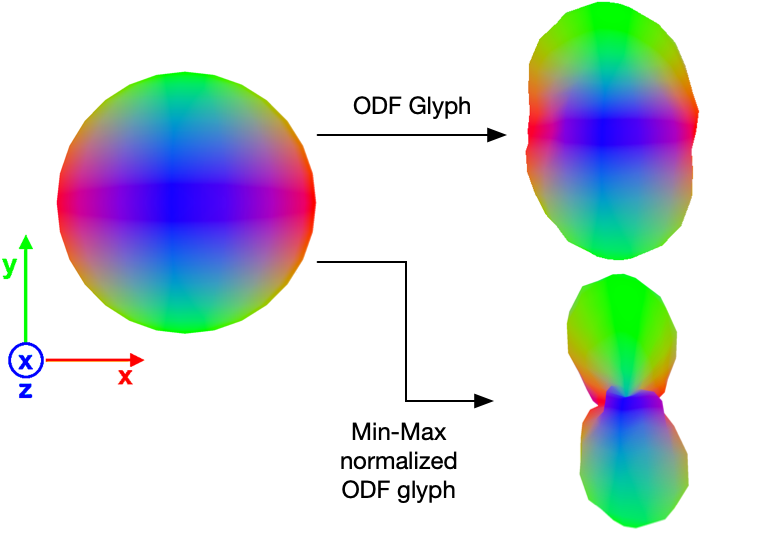
\includegraphics[width=.45\linewidth, angle=0]{figs/SphericalMeshModulation.png}
    \caption{Spherical polar plots of an ODF and its min-max normalized version. The RGB color mapping follows Eq. \ref{eq::glyph_color}.}
    \label{fig::intro_glyph}
\end{figure}
%The normalized version has a more pronounced orientational structure. 

%\sout{These advanced methods that requires a HARDI acquisition, which will be called in this work as HARDI methods, aims to reconstruct} \textcolor{blue}{Tuch showed that when the angular acquisitions are uniform, one can synthesize from the samples} an orientation distribution function (ODF) that represents the diffusion process. \sout{Some of them are}\textcolor{blue}{This function is} model-free\sout{, which}\textcolor{blue}{It} estimates the diffusion displacement from the Fourier relation between the DW-MRI signal to its respective diffusion displacement \cite{TuchQBall2004, wedeen2005,  yeh2010}\sout{ and others are}\textcolor{blue}{Tournier presented a} model-based \textcolor{blue}{approach}\todo{It is not clear the underlying model! FOD, fiber orientation density???}\textcolor{red}{, where they model the underlying fiber signal obtained by its respective decay on the diffusion acquisition \cite{tournier2007}.}

%\sout{These advanced methods that requires a HARDI acquisition, which will be called in this work as HARDI methods, aims to reconstruct} \textcolor{blue}{Tuch showed that when the angular acquisitions are uniform, one can synthesize from the samples} an orientation distribution function (ODF) that represents the diffusion process. \sout{Some of them are}\textcolor{blue}{This function is} model-free\sout{, which}\textcolor{blue}{It} estimates the diffusion displacement from the Fourier relation between the DW-MRI signal to its respective diffusion displacement \cite{TuchQBall2004, wedeen2005,  yeh2010}\sout{ and others are}\textcolor{blue}{Tournier presented a} model-based \textcolor{blue}{approach}\todo{It is not clear the underlying model! FOD, fiber orientation density???}\textcolor{red}{, where they model the underlying fiber signal obtained by its respective decay on the diffusion acquisition \cite{tournier2007}.}

%An ODF consists in an association of a set of directions, each one of \sout{them}\textcolor{blue}{which} \textcolor{blue}{is} represented by a unity vector $\bm{u}$, to a scalar $\psi(\bm{u})$. The most common approach to represent an ODF by a glyph is through the spherical polar plot. In this category of a glyph, a \todo{Reference to normalized ODF}normalized \sout{version of the} ODF deforms a sphere accordingly to \sout{the equation}\textcolor{blue}{Eq.} \ref{eq::normglifo}:

\begin{equation}
\label{eq::normglifo}
    R(\bm{u}) = \frac{\psi(\bm{u}) - min(\psi(\bm{u}))}{max(\psi(\bm{u})) - min(\psi(\bm{u}))}
\end{equation}

%Fig. illustrates comparatively a spherical polar plot generated by an ODF and its min-max normalized version. 
Note in Figure \ref{fig::intro_glyph} the use of color to enhance the diffusion orientation. A simple color mapping, commonly used by the DWI community, is applied to the unit vector  $\bm{u} = (u_x, u_y, u_z)$ to get the RGB components, as defined in Eq. \ref{eq::glyph_color}.

\begin{equation}
\label{eq::glyph_color}
    r = |u_x| ~~~~ g = |u_y| ~~~~ b = |u_z|, 
\end{equation}

where, concerning anatomical planes, the red color ($r$) represents the mediolateral direction, the green ($g$) refers to the anteroposterior direction, and the blue ($b$), inferior-superior direction.

%where $R(\bm{u})$ is the length of a deformed sphere in the direction $\bm{u}$.

These glyphs provide a coherent visualization of local diffusion in each DWI sample. Researchers use them to validate imaging methods \cite{descoteaux2007_QBI,  TuchQBall2004,tournier2007,Tournier2004DirectEO, tuch2002,  yeh2010} and assess the local relationship among scanned diffusion data and the estimation of the underlying fiber architecture \cite{cho2008, daducci2014,descoteaux2007, vega2009,Vaillancourt2015}. %The FODs extracted from an imaging method applied to a DWI acquisition are used as input of fiber tracking algorithms. %The conjecture of the possibility of brain connectivity from the DWI acquisitions motivates this research area's main motivation.

It is highly desirable to visualize and explore HARDI data in an interactive way. It would improve the brain connection research quality and help to move advanced diffusion imaging into clinical practice~\cite{Shapey2019}. However, the high dimensionality of ODF has been an obstacle, especially when one wants to take advantage of GPU's capacity and performance \cite{peeters2009}.

Peeters et al. \cite{peeters2009} advocated that the ray-casting approach is more appropriate to deal with CPU-GPU data transfer bottleneck. The amount of data to be transferred from CPU to GPU could be greatly reduced by only passing the position and coefficients of the ODF glyph's geometric representation. Besides, in the ray-casting approach, the glyph rendering quality is not dependent on the mesh resolution as triangle-based one. However, Voltoline and Wu showed that the advanced GPU features could make the triangle-based rendering competitive with the ray-casting one, with the advantage of avoiding the root-finding problem and exploring the outperformance of the triangle hardware graphics accelerator.

%, namely instanced rendering, transform feedback, tessellation shader, and indirect rendering,

%\textcolor{magenta}{In this work, we explore instance rendering }
%\todo{Insert a figure to help in understanding.}These glyphs\textcolor{blue}{, as illustrated in Fig~\ref{???},} \sout{give}\textcolor{blue}{provide} a clear visualization of local \sout{information in} diffusion \sout{imaging methods} \textcolor{blue}{in each voxel}. \sout{It is used by} \todo{References?}Researchers use them to \todo{???}\textcolor{red}{assess the acquisition quality,} \sout{attest the validity of}\textcolor{blue}{validate} an imaging method, \sout{the adequability of it given an acquisition} and \sout{the} check the relationship between the \textcolor{blue}{applied} imaging method \sout{used with} \textcolor{blue}{and the} fiber reconstruction algorithms called tractography.


%\todo[inline]{I suggest writing motivation to this work: the challenging remaining problems and the one you are supposed to solve.}

In this work, we present an interactive GPU-accelerated triangle-based rendering scheme for HARDI ODF glyphs. We applied the GPU-based superquadric glyphs rendering principle proposed by Voltoline and Wu \cite{voltoline2021}.
%\sout{The gains of performance are given by decreasing the amount of data traffic CPU-GPU by taking out redundant information on each drawing request. This is achieved by using instance rendering.}
%In this work, we present a\textcolor{blue}{n interactive GPU-accelerated} rendering scheme \sout{that aims to, given samples of ODFs associated with a spherical mesh, we} \textcolor{blue}{to} render a set of spherical polar plot\textcolor{blue}{s from ODF samples}. \textcolor{blue}{Inspired by Voltoline and Wu's work, we applied instance rendering and transform feedback to reduce the CPU-GPU data traffic.}\sout{The gains of performance are given by decreasing the amount of data traffic CPU-GPU by taking out redundant information on each drawing request. This is achieved by using instance rendering.}
%\todo{is rendering necessary for visualization?}\sout{This rendering scheme, integrated with visualization systems to diffusion images, can be a powerful tool for researchers in the area to assess a set of local diffusion profiles and improve their understanding of advanced methods for diffusion imaging.}
The paper is organized into six sections. In Section \ref{sec::related_work}, we discuss the related works; in Section \ref{sec:superquadric_rendering}, we briefly present the interactive multimodal rendering pipeline for superquadrics proposed by Voltoline and Wu; in Section \ref{sec::odf_glyph_rendering}, we discuss our proposed modifications to make their pipeline appropriate for ODF glyph rendering; in Section \ref{sec::results}, we show the rendering algorithm performance; and in Section \ref{sec::conclusions}, we conclude the work with discussion.

\paragraph*{\textbf{Contributions}}

This paper's main contribution is a GPU triangle-based rendering algorithm for ODF glyphs. We discuss a strategy for dealing with ODF data's high dimensionality that has less impact on memory bandwidth and latency. We show that the glyphs can be rendered at interactive rates.

%\todo{Redundant text. Instead, write the expected contribution.}\sout{The integration of this rendering scheme in a DW-MRI visualization can be  It improves the understanding of the output result of an diffusion imaging method applied to DW-MRI, as well as provide an a visual information of the underlying model where directional information of fibers is extracted to be used on brain fiber reconstruction. The real time factor can improve the visual interactivity of the research in the area.}

%We ask authors to follow this guideline and make paper look exactly like as this document. The easiest way to do this is simply to download a template from \cite{jou01a} and replace the content with your own.

%\section{Background}

\section{Related work}
\label{sec::related_work}

%\todo[inline]{You must show briefly why the works are related to your work. Which aspects did you take advantage of in your work? If you want to detail a specific work, open another section.}

%Polygons based glyph rendering schemes is an area that has not been much explored by the HARDI community. Shattuck et al. \sout{\cite{shattuck2008} showed results of a polygon based approach} \textcolor{blue}{presented} in \sout{his}\textcolor{blue}{their} work \textcolor{blue}{\cite{shattuck2008} the rendering of ODFs as spherical meshes of 225 vertices and 2 million triangles in 10 FPS.}\sout{ and, at that time, the result reported by them was 10 FPS when using a spherical mesh of 225 vertices, with 2 million triangles being rendered.} The authors \sout{do}\textcolor{blue}{did} not \sout{explain} detail\sout{ed} their rendering scheme\sout{ and imply that they were not programming the GPU. It is worth mentioning that instance rendering was not released back then}.

 Despite the recognized relevance of interactive rendering of HARDI data, the community has not explored this issue much. Interested in performance, we will limit ourselves here to works that exploit the GPU resources. Two major approaches are found in the literature for rendering glyphs. One is based on ray-casting, where each glyph's geometry is represented by a function or algebraic expression \cite{peeters2009, almsick2011}. The other is based on the mesh's rendering with the glyphs' geometry approximated in polygonal meshes \cite{shattuck2008}.
 
 %\todo{S\~ao se\c{c}\~oes curtas ... N\~ao vle a pena de dividi-las.}
 

Shattuck et al. \cite{shattuck2008} tessellated a polar representation of an ODF with triangles by subdividing its polar domain and generating its shape on the CPU from an analytical function over this domain. The glyphs are rendered per slice. Whenever the mesh's modeling and viewing parameters changed, the glyphs' vertices were recomputed and resent to the GPU. The performance reported was ten frames/sec for a brain slice using a spherical mesh of 225 vertices per glyph, corresponding to approximately 2 million triangles. We explore, in this work, modern GPU features to improve rendering performance and GPU-memory usage. %and \todo{\textcolor{green}{The Raphael's concept of determining the mesh as function of how many pixels is occupied by a voxel is not something I am applying. In this work, the spherical mesh is fixed. That being said, there is a opportunity to do it} screen occupancy.}

%ALGO RELEVANTE: ESSE TRABALHO DO SHATTUCK É O ÚLTIMO DA ÁREA QUE TEM ALGUMA COISA A VER COM O MEU, QUE É RENDERIZAR GLIFOS HARDI EM TEMPO REAL VIA POLIGONOS.

% \sout{ and imply that they were not programming the GPU. It is worth mentioning that instance rendering was not released back then}.

%\subsection{Raycasting-based ODF glyph rendering}

Peeters et al. \cite{peeters2009} proposed a ray casting approach to render glyphs. On the CPU, the center, the radius of the bounding sphere, and the bounding cube per spherical polar plot were computed. On the GPU, the raycasting algorithm is executed per pixel in the fragment shader. If the ray shot from a pixel through the view volume did not intersect the bounding sphere, the fragment was discarded. Otherwise, they performed a linear search, with discrete steps, for the intersection with ODF along the shot ray. They achieved better performance than the algorithm presented by Shattuck et al. \cite{shattuck2008}. Almsick et al. \cite{almsick2011} further improved the intersection search using the \textit{regula falsi} numerical method and bounding cylinders aligned with the viewing axis. They achieved higher time performance without sacrificing the rendered glyph quality, reporting that 9,000 glyphs could be generated at 30 fps. Nevertheless, the critical issue of intersection finding's accuracy and efficiency with an ODF along the shot ray remained. When the ray was almost parallel to the glyph, many iterations might incur in some threads. The triangle-based rendering we applied in this work does not suffer from the root-finding problem.


%They also compared their approach to the polygon based rendering scheme proposed by Shattuck et al. \cite{shattuck2008}. 

%adapted the seven-pass multimodal rendering algorithm proposed by Voltoline and Wu \cite{voltoline2021} to render spherical polar plots of high dimensionality.

%\subsection{Triangle-based DTI's superquadric interactive rendering}
%\label{ssec:superquadric_rendering}

Voltoline and Wu \cite{voltoline2021} proposed a real-time triangle-based rendering scheme for superquadric tensor glyphs \cite{Kindlmann2004}. They explored several modern GPU features to achieve this goal, such as instanced rendering, transform feedback, adaptive triangular approximation of glyphs, and indirect rendering to render glyphs computed from DTI data uploaded to the GPU. However, unlike the superquadric glyphs, the data associated with ODF glyphs are much larger, making it inviable to store it on the GPU. Thus, we must devise a way to subdivide the large volume into a set of bricks that fit into the GPU memory for the glyphs to be rendered.

%http://people.seas.harvard.edu/~jbeyer/files/documents/beyer_star_large_volren_14.pdf

%Section \ref{sec:superquadric_rendering} gives a brief overview of their proposal. \sout{These results influenced us to adapt their scheme into our proposed HARDI glyph rendering scheme}


%\textcolor{blue}{We showed in this work how to structure the ODF data in a compliant way with the superquadric tensor data so that the ODF data can take advantage of \sout{the same} \textcolor{magenta}{a similar} GPU processing flow}.


%\section{Rendering scheme}
\section{Superquadric Glyph Rendering}
\label{sec:superquadric_rendering}

%\todo{For the sake of efficiency, three stages: (1) Compute the visible voxels (number of glyphs); (2) Estimate the coverage of glyphs in pixels (resolution of glyphs); (3) rendering.}

In this section, we detail the GPU-based DTI superquadrics rendering algorithm proposed by Voltoline and Wu \cite{voltoline2021}, and the ideas we have brought to our work.

%!!CORRIGIR ISSO AQUI.TROCAR b0 POR ANISOTROPIA
They propose a rendering pipeline for triangle-based superquadric glyphs overlaid over their corresponding anatomical T1-weighted MRI (T1wMRI) voxels. The DWI's $b0$ volume, its corresponding anatomical T1wMRI, and the rigid matrix that co-registers the two volumes are uploaded to the GPU \cite{ting2014}.

%\sout{In order to make their approach interactive, they propose strategies to keep the CPU-GPU data traffic minimum, how to minimize the occupancy of the glyph's data on GPU's memory and how to make the number of triangles on each glyph's mesh adaptive as a function of its size.}

%\todo{The following description is confusing.}

The rendering algorithm is divided in three stages: rendering the co-registered DWI and T1wMRI; detecting visible voxels and estimating the maximal coverage of the glyph's projection in pixels to estimate the mesh's resolution; rendering the visible glyphs in the estimated resolution. %and minimize the occupancy of glyph's data on GPU's memory given the estimated mesh.

Because the highest OpenGL version that Mac OSX can support is 4.1, they unfolded the one-pass voxel coverage compute shader into a four-pass algorithm involving rasterization-based vertex, geometry, and fragment shaders. The transform feedback buffer was applied to avoid the inter-pass data transfer between the CPU and the GPU. Also, they showed how to use the additive blending mechanism to get the maximum amount of pixels ($max_p$) on which a voxel projects.  Based on $max_p$, they developed a heuristic to estimate the mesh's resolution.

%\sout{In order to detect on-screen voxels and estimate the mesh resolution, they propose an estimation of the volume's voxels coordinates on the onscreen buffer of the rendered volume as a transform feedback buffer. Furthermore, this buffer is also used to do the mesh's amount of triangles computation, which is a function of the maximum amount of pixels ($max_p$) containing one single voxel. The mesh's amount of triangles is the same for all glyphs and is set in each drawing request in GPU's tessellation shader.}

They used indirect instance rendering to minimize draw calls and glyph data occupancy on the GPU memory. Providing each instance with unique superquadric parameters, they showed that only a single draw call of a point was enough to trigger a tessellation shader for building a skeleton of the base superquadric glyph from a quad patch. Then, each glyph is translated into the corresponding voxel's center in the volume space, using the instanced geometric transformation.

% It consists in an uniform discretization of the spherical coordinates $(\phi, \theta)$ in the interval $[0,2\pi], [0, \pi]$ respectively.


 %The amount of subdivisions is a function of the largest amount of pixels occupied by a volume's voxel. The higher the amount of pixels by occupied by a voxel, the bigger is the shape of the superquadric, and the work proposes a GPU-based algorithm to increase the resolution of the superquadric's mesh, accordingly.
 
 %\todo{For the sake of GPU implementability and efficiency, three stages: (1) Compute the visible voxels (number of glyphs to be sent); (2) Estimate the coverage of glyphs in pixels (resolution of glyphs); (3) rendering.}

\section{ODF Glyph Rendering}
\label{sec::odf_glyph_rendering}

%\subsection{Overview}

The ODF associated to a voxel is typically represented by a set of $N$ diffusion samples $[R(\bm{u_1}), R(\bm{u_2}), ..., R(\bm{u_{N-1}}), R(\bm{u_{N}})]$, where $R(\bm{u_i})$ is calculated using Eq. \ref{eq::normglifo}. An ODF glyph synthesizes all these samples in a geometric shape by displacing each point $P_K$ of a base spherical mesh by the corresponding scalar $R(\bm{u_k})$, where $\bm{u_k}$ is the diffusion direction parallel to the normal vector at $P_K$. All the ODF samples are pre-processed on the CPU and accessible by their respective voxel indices. 

Because of GPU memory limitation, we applied the display-aware approach proposed by Voltoline and Wu \cite{voltoline2021} to get the set of $D = [d_1, d_2, ... d_M]$ visible voxel indices and suggest only sending their respective ODFs to the GPU for instance rendering, as illustrated in Fig. \ref{fig::vmtk_simplified}. It, however, caused the CPU-GPU data transfer penalty due to frequent changes in rendered images associated with the user's interactions. Thus, in this section, we present strategies to tackle the transfer at interactive rates.

\begin{figure}[ht]
    \centering
    %\rule{6cm}{3cm}
    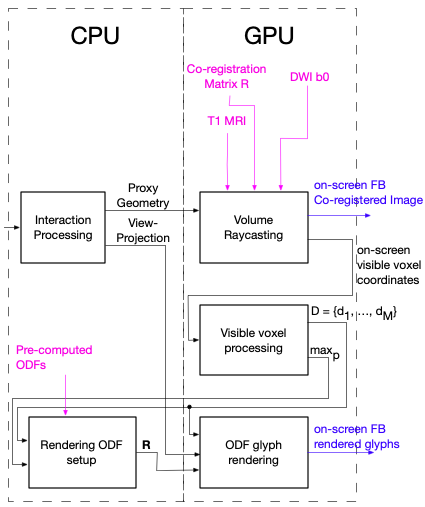
\includegraphics[width=1.0\linewidth, angle=0]{figs/rendering_scheme/fluxograma_glifosVMTK_5.png}
    \caption{Multimodal rendering for ODF glyphs. The blue color represents the output to be drawn on the framebuffer (FB); the magenta color refers to pre-computed elements. The volume raycasting and visible voxel processing stages are described in \cite{voltoline2021}. The Rendering ODF setup and ODF glyph rendering stages are described in section \ref{sec::odf_glyph_rendering}.}
    \label{fig::vmtk_simplified}
\end{figure}

Our key solution was to minimize data volume by exploring the visual perception resolution, GPU instancing, ODF data symmetry, and GPU texture memory allocation politics. Section \ref{ssec::glyph_resolution} describes the base spherical mesh that is deformed by each ODF glyph's samples. In Section \ref{ssec::glyph_attributes}, we describe the attribute layout that optimizes the GPU memory usage and accesses.

%http://people.seas.harvard.edu/~jbeyer/files/documents/beyer_star_large_volren_14.pdf

%The strategy showed in our work consists in, , reducing the CPU-GPU data traffic and keeping the . These indices set can refer to a slice, for example.

%\sout{In an application that integrates the glyphs with DWI and anatomical visualization, we advise the reader to use this work integrated with the on-screen volume's voxel detecting scheme and the on-screen size estimation in Voltoline and Wu's \cite{voltoline2021} work. In subsection \ref{ssec::multimodal}, we briefly mention the integration of our work on the multimodal rendering scheme and report its respective rendering FPS.}\textcolor{magenta}{As we show in the section !!REFER HERE TO AN EXPERIMENT WHERE BOTH ARE BE INTEGRATED}

%Then, we use the onscreen voxel detection, return to CPU its data, extract the voxels' respective index set, organize the data and send to GPU to render.

%Our biggest concern has been the CPU-GPU data traffic, which consists mainly on ODF's samples, and we show strategies to minimize it.

%In our work, we show a rendering scheme that the input consists in a set of voxel indices, whose glyphs are to be rendered and its data, which consists of its translation matrix to the volume space and ODF data is pre-computed on CPU.



%Worth noting that the scheme is also applicable in slice rendering, where the 



%namely instanced rendering, transform feedback, tesselation shader, and indirect rendering, could make the triangle-based rendering competitive with the ray-casting one,


%The number of samples that customize a glyph is usually in the hundreds \cite{TuchQBall2004, yeh2010}, yielding a high amount of data sent to GPU in every drawing request for multiples of them. Thus, the suggested procedures in the subsection \ref{ssec::datastruct} consists on strategies to minimize the data-traffic and are crucial to the scheme.

% and, in the subsection \ref{ssec::optimization}, we discuss an optimization that can be done in symmetrical ODFs.

%The input of the rendering scheme consists in two set of elements: the set positions in the scene and a set of ODF profiles that .

%We divide the rendering scheme in precomputation and drawing request. The precomputation  refers to the part of the rendering scheme that is done at the beginning of scheme and only once, and the 

%\todo[inline]{An overview of the proposal. It could be a flowchart}





%\subsection{Applicability on ODF glyph rendering}

%\subsection{CPU and GPU Algorithms for Rendering Overview}

%\label{ssec::rendering}
%\subsubsection{CPU}
%\begin{enumerate}
%    \item Set the base geometry in run time;
%    \item Update translation attributes buffer with the $M$ voxel indices set of glyphs requested to be rendered and send to GPU;
%    \item Setup the requested voxels' ODF data set and send to GPU.
%\end{enumerate}

%\subsubsection{GPU}
%Vertex Shader:
%\begin{enumerate}
%    \item Lookup the coefficient that map the base geometry vertex to the glyphs surface;
%    \item perform the translation of the vertex;
%    \item apply view-projection transformation;
%    \item compute color as a function of the spherical mesh vertex accordingly to Eq. \ref{eq::glyph_color} and send to the fragment shader.
%\end{enumerate}

%Fragment Shader:
%\begin{enumerate}
%    \item Set the output color as the rasterized color set in the vertex shader.
%\end{enumerate}






%\subsection{Glyph base geometry}
\subsection{Glyph geometry}
%\subsection{Initialization}
\label{ssec::glyph_resolution}

%The glyphs consist of spheres with each one of its radius points deformed by its respective ODF value.

%\sout{The geometric model consists in setting up a base spherical mesh and a scaling factor that fits the glyphs to the visible voxels' dimensions so the user can afford to maximize screen occupancy. The scaling factor is given by }
%\begin{equation}
%\label{eq:spacings}
%mS = min(spacing_x, spacing_y, spacing_z)
%\end{equation}



%\todo[inline]{It is not clear the data stored in the index buffer? The indices of the coordinates of each vertex? Did you create an vertex buffer object and indexing its elements to improve the memory usage?}

The ODFs are sampled on a base spherical mesh $(\Pi, I)$, which consists in a unit sphere centered at the origin, discretized in N points, $\Pi = \{P_1, P_2, \dots, P_N\}$. We associate to each point in $\Pi$ an entry of the set of indices $I$, which reference the point's attributes, so we store these attributes only once, even if used many times in rendering the mesh triangles. We establish two conditions for the mesh's data structure, given by $[P_1, P_2, \dots, P_N]$, which we take advantage of the ODF data symmetry, and make the mesh adaptive to viewing parameters. These conditions have a direct impact on the CPU-GPU data traffic, as discussed further in Subsection \ref{ssec::glyph_attributes}. Then, in the application, we use the two-powered tessellation order of the icosahedron derived meshes, which satisfy the established conditions and derive a heuristic expression that set one of these meshes at run time to be the glyphs' base geometry as a function of the viewing parameter $max_p$.

%The first condition allow us to decrease the data storage of ODF samples and its per-glyph CPU-GPU data traffic from the whole sphere to the half; and the second makes possible the exploration of the visual perception by allowing the reduction of the glyphs' base geometry resolution by using sub-meshes of the base spherical mesh, decreasing not only the GPU processing demands, as the per-glyph CPU-GPU data traffic.

The first condition aims to take advantage of HARDI ODF's symmetry ($R(\bm{u}) = R(-\bm{u})$). We suggest that the base mesh $(\Pi, I)$ is symmetrical with respect to the origin, i.e. $P \in \Pi \implies -P \in \Pi$, and its respective data structure is organized in the sequence $[P_1, -P_1, P_3, -P_3, \dots, P_{N-3}, -P_{N-3}, P_{N-1}, -P_{N-1}]$, where $P_{2K+2} = -P_{2K+1}$, $(0 \leq K \leq \frac{N-2}{2})$.

The second condition aims to make the glyph's base geometry adaptive as a sub-mesh of the base spherical mesh $(\Pi, I)$. Let $k$ be the number of sub-meshes of $(\Pi, I)$, where each sub-mesh is denoted by $(\Pi_i, I_i)$,  $(0 \leq i < k)$, and the number of vertices of each sub-mesh increases with its sub-index, i.e. if  $(0 \leq i < j < k)$, implies $|\Pi_j| > |\Pi_i|$. We suggest that, each sub-mesh $(\Pi_i, I_i)$ is symmetrical across the origin and the first $|\Pi_i|$ elements in  $\Pi$'s data structure corresponds to the elements of $\Pi_i$. Note that the condition establishes, for $i$, $j$ such $0 \leq i < j < k$ implies that $\Pi_i \subset \Pi_j$.

The category of spherical meshes that we chose that satisfies the conditions stated are derived from the two-powered tessellation order of the icosahedron. The algorithm to obtain the $2^k$-th tessellation order is an iterative process repeated $k$ times that starts with an icosahedron. Each triangle is subdivided in four in each iteration, where the new vertices are computed as the projection of each median points of each pair of connected vertices onto the sphere. Thus, the $2^k$-th tessellation order vertices set contains all vertices of the anterior iterations, and, in addition to that, they are all symmetrical with respect to the origin. The algorithm to obtain this category of spherical mesh can be found in \cite{luna2012}.

Therefore, assigning $(\Pi, I)$, $2^{k}$-th tessellation order of the icosahedron as the base geometry and keeping each index set at each iteration, we have a set of $k$ sub-meshes $(\Pi_0, I_0), (\Pi_1, I_1), ..., (\Pi_{k-1}, I_{k-1})$ as the $1^{st}$, $2^{nd}$, ... $2^{k-1}$-th tessellation order.

%The vertices subset property can be corroborated by the fact that tessellation of order $2^k$ consists of a subdivision of each triangle of the $2^{k-1}$-th tessellation in four.



The vertices and amount of triangles and the expression for the vertices and triangles number for each $2^k$ tessellation are in Table \ref{tab::icosahedron_set}. In practice, we recommend $k$ to be equal to 3 or 4, at most. Values of above those may incur a prohibitive amount of memory for pre-computed ODF samples in a DWI.

\begin{table}[]
\centering
\begin{tabular}{|c|c|c|c|}
\hline
\textbf{Order} & \textbf{\#Vertices} & \textbf{\#Triangles} \\ \hline
1              & 12                 & 20                  \\ \hline
2              & 42                 & 80                 \\ \hline
4              & 162                & 320                 \\ \hline
8              & 642                & 1280                \\ \hline
16             & 2562               & 5120                \\ \hline
$2^k$          & $10\times 4^k + 2$ & $20\times 4^k$           \\ \hline
\end{tabular}
\caption{Amount of vertices and triangles of 2-powered order tessellation of the icosahedron.}% For $k<n$, the vertices on the tessellation $2^k$ is a subset of $2^n$.}
\label{tab::icosahedron_set}
\end{table}

Assigning the base spherical mesh $(\Pi, I)$ to be the $16^{th}$ order of tessellation of the icosahedron, the meshes of order $1$, $2$, $4$ and $8$ are used as sub-meshes. Thus, the base spherical mesh's data structure that satisfies the two conditions is that the first 12 elements corresponds to the icosahedron's vertices, 42 elements correspond to the $2^{nd}$ tessellation order, the 162 first elements corresponds to the $4^{th}$ tessellation order, the 642 first elements corresponds to the $8^{th}$ tessellation order, and, additionally, the symmetrical points are grouped in sequence in memory. %Thus, we established $k-1$ sub-meshes of $(\Pi, I)$. \textcolor{red}{In practice, we recommend $k$ to be equal to 3 or 4, values of above that may incur a prohibitive amount of memory for ODF samples in a DWI.}

The mesh $(\Pi, I)$ and the indices set that triangulates all the sub-meshes are sent to GPU once. Aiming at greater efficiency without compromising the meshes' visual quality, we adaptively choose the base geometry among these meshes by a heuristic procedure based on $max_p$ at run time.

The mesh selection follows Voltoline and Wu's trade-off $\tau > 8\sqrt{max_p}$; $max_p > 0$ \cite{voltoline2021}, where $\tau$ is mesh amount of triangles and $max_p$ the maximum amount of pixels containing a single DWI's voxel. This trade-off establishes the minimum number of triangles that do not sacrifice the image quality. Replacing this ratio with the expression of the amount of triangles as a function of icosahedron's tessellation order and mapping the icosahedron to be the lowest resolution mesh to be used, we derive $t$ ($t \leq k$) in Eq. \ref{eq::icosa_order} as the chosen $2^{t}$-th tessellation order of the icosahedron:

\begin{equation}
\label{eq::icosa_order}
     t = \lceil \frac{1}{2}\log_2{(\frac{2}{5}\sqrt{max_p} + 1)} \rceil
\end{equation}

%where it chooses the base geometry among the available based on the least amount of triangles that satisfies the trade-off.



%Aiming at greater efficiency without compromising the meshes' visual quality, we adaptively chose the mesh resolution among $t$ sub-meshes of $(\Pi, I)$ at run time as a function of $max_p$. Thus, we suggest that, for each $(\Pi_i, I_i)$ $(1 \leq i \leq t)$ lower resolution mesh, where $\Pi_i \in \Pi$, the first $|\Pi_i|$ elements in the $\Pi$'s data structure corresponds to $\Pi_i$'s vertices.

%Let us define a set $\Delta$ of $k-1$, sub-meshes where each element $\delta_i = (\tau_i/8)^2$; where $i = 1, 2, ..., k-1$ refers to the $2^{nd}$, $4^{th}$, ..., $2^{k-1}$-th tessellation order of the icosahedron. Keeping the minimum amount of triangles, given a $max_p$, we suggest a procedure that chooses one of the $k$ meshes that has the lowest amount of triangles that satisfies the trade off:

%\textcolor{red}{The category of spherical meshes that we chose that satisfies the conditions stated are derived from the two-powered tessellation order of the icosahedron \cite{???}.} 
%They are symmetrical and present the following property: for $k < n$, the vertices of the $2^{k}$ order tessellated icosahedron is a subset of $2^{n}$.



For the $2^t$-th tessellation order chosen as a base geometry, one must be attentive to two procedures to select the mesh at run time. The first consists in the activation of its respective index buffer for the draw call. The second consists in setting the amount of per-glyph data sent to GPU as a function of its vertices, as discussed further in the subsection \ref{ssec::glyph_attributes}.

Finally, we suggest scaling the normalized base mesh by the scaling factor $mS$ to afford the maximal screen occupancy.

\begin{equation}
\label{eq:spacings}
mS = min(spacing_x, spacing_y, spacing_z)
\end{equation}

where $spacing_x$, $spacing_y$, $spacing_z$ are the spacing between adjacent DWI samples in the x-, y- and z-axis, respectively.


%\subsection{O QUE FAZER COM ISSO?}
%The vertices subset property can be corroborated by the fact that tessellation of order $2^k$ consists of a subdivision of each triangle of the $2^{k-1}$-th tessellation in four. These four triangles vertices' are formed by six points: three of them are the same of the base triangle from $2^{k-1}$-th order, and the other three are derived from these points as they are each pair's projection of the median points onto the sphere as illustrated in Fig. \ref{fig::subdivision_icosahedron}. Table \ref{tab::icosahedron_set} shows the number of vertices and triangles of each tessellation order.





% \begin{figure}[htb]
%     \centering
%     %\rule{6cm}{3cm}
%     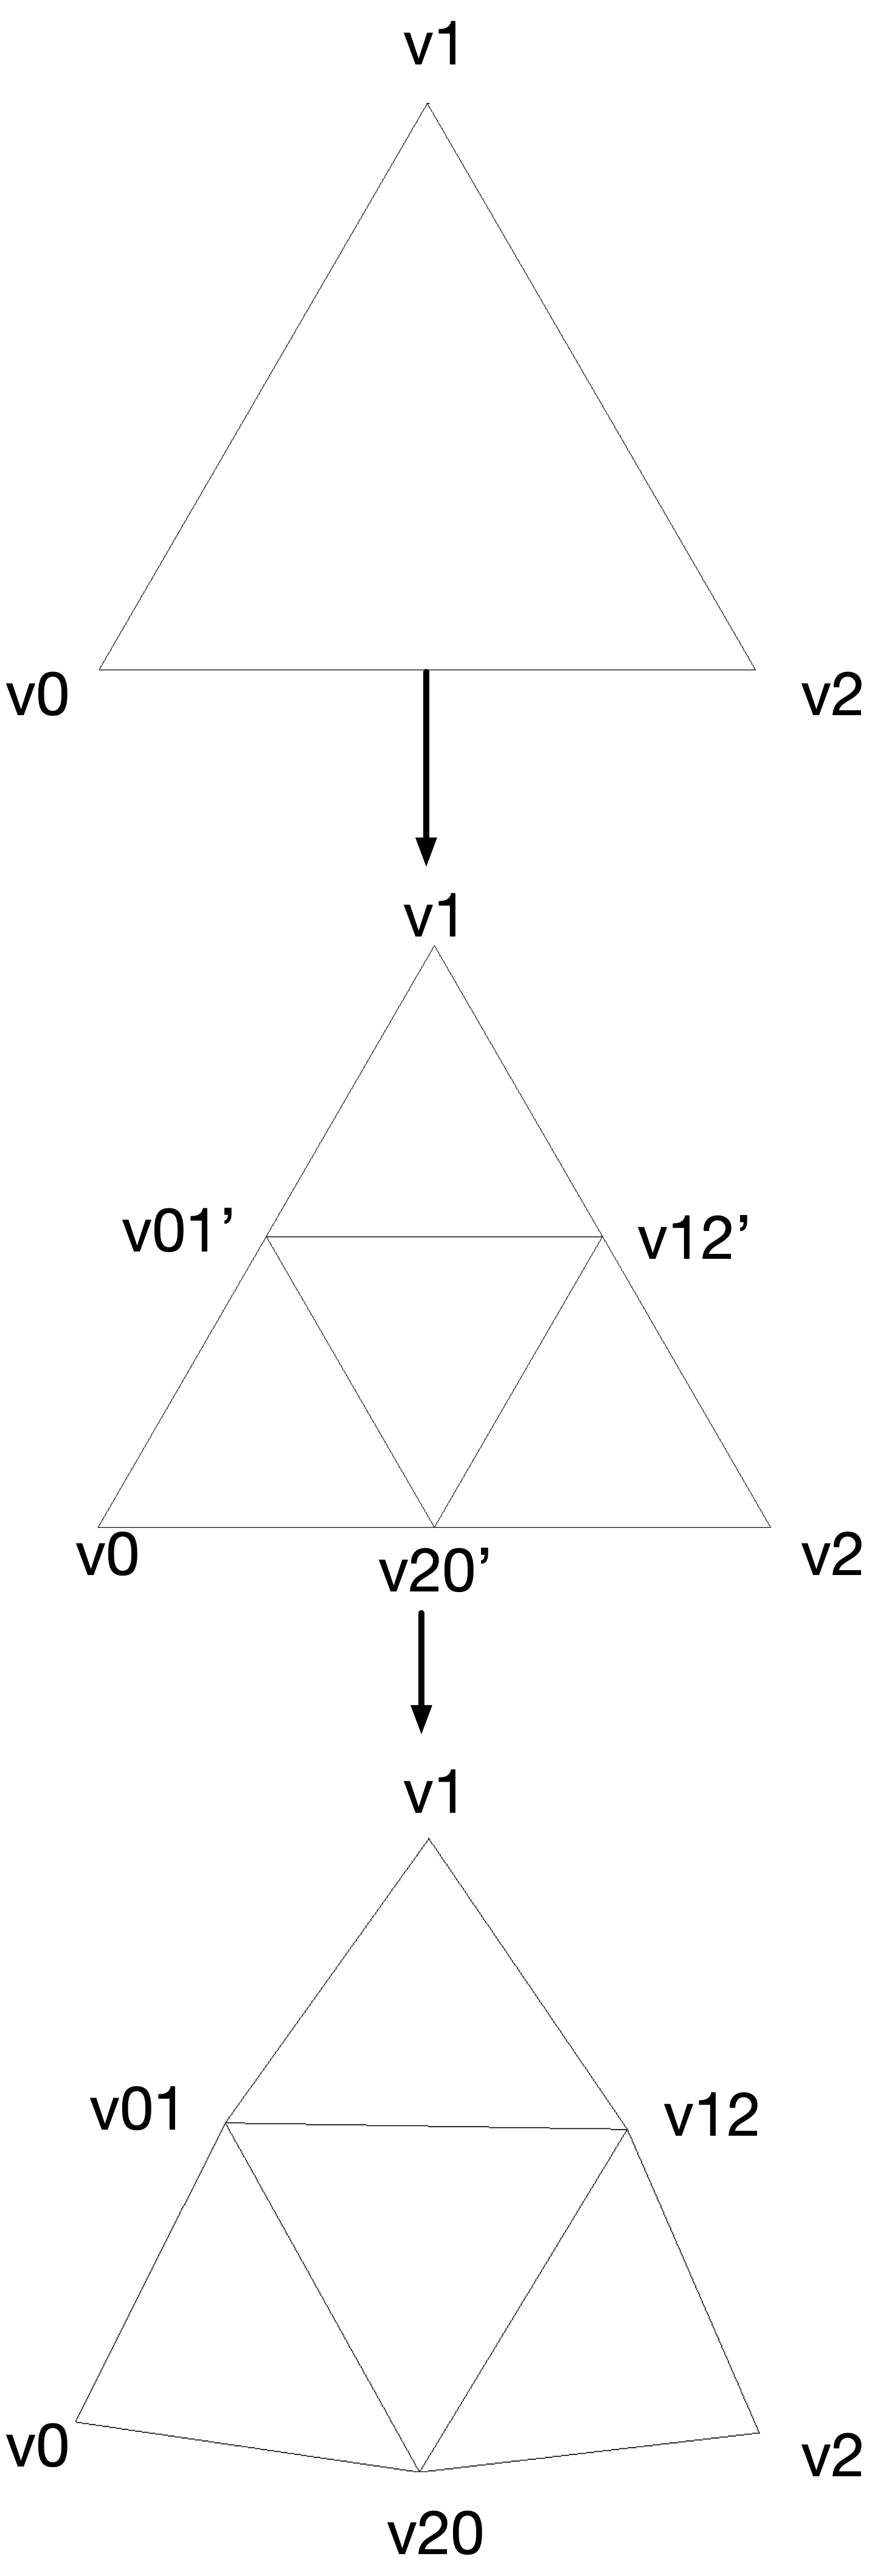
\includegraphics[width=.45\linewidth, angle=0]{figs/icosahedron_example/ico_subdivision_V.png}
%     \caption{Triangle subdivision to form a $2^k$-th order of tessellation of the icosahedron from a $2^{k-1}$-th order. The triangle formed by v0, v1, and v2 is subdivided into four triangles, where the median points v01', v12'and v20' are computed, and their projections on the unit sphere v01, v12, and v20 are added into the vertices set.
%     }
%     \label{fig::subdivision_icosahedron}
% \end{figure}





%\textcolor{blue}{Aiming at greater efficiency without compromising the meshes' visual quality, we adaptively chose the mesh resolution among $t$ sub-meshes of $(\Pi, I)$ at run time as a function of $max_p$. Thus, we suggest that, for each $(\Pi_i, I_i)$ $(1 \leq i \leq t)$ lower resolution mesh, where $\Pi_i \in \Pi$, the first $|\Pi_i|$ elements in the $\Pi$'s data structure corresponds to $\Pi_i$'s vertices.}





%Let us define a set $\Delta$ of $k-1$, sub-meshes where each element $\delta_i = (\tau_i/8)^2$; where $i = 1, 2, ..., k-1$ refers to the $2^{nd}$, $4^{th}$, ..., $2^{k-1}$-th tessellation order of the icosahedron. Keeping the minimum amount of triangles, given a $max_p$, we suggest a procedure that chooses one of the $k$ meshes that has the lowest amount of triangles that satisfies the trade off:




%\begin{enumerate}
%    \item if $max_p \leq \delta_1$, choose $2^{nd}$ tessellation order;
%    \item if $\delta_{1} < max_p \leq \delta_{k-1}$, choose the $2^{t}$-th tessellation order such that $\delta_{(t-1)} < max_p \leq %\delta_{t}$;
%    \item if $max_p > \delta_{k-1}$, choose $(\Pi, I)$ - $2^{k}$-th tessellation order
%\end{enumerate}

%\textcolor{blue}{For the mesh $(\Pi_i, I_i)$ chosen, one must be attentive to two procedures to select the mesh at run time. The first consists in the activation of its respective index buffer for the draw call. The second consists in changing the amount of per-glyph data sent to GPU, as discussed further in the subsection \ref{ssec::glyph_attributes}.}



%\sout{The mesh forms the base geometry of all glyphs and is sent to the GPU once.}

%\sout{For the sake of performance, we suggest that the mesh used is symmetric, and its points form lower resolution spherical meshes.}

%\sout{The mesh is symmetrical if $P \in \Pi \implies -P \in \Pi$. We also suggest that the data structure sent to GPU has the pair of symmetrical points grouped, as $[P_1, -P_1, P_3, -P_3, \dots, P_{N-3}, -P_{N-3}, P_{N-1}, -P_{N-1}]$, where $P_{2K} = -P_{2K-1}$, $(1 \leq K \leq N/2)$.}



%\todo[inline]{Os par\'agrafos abaixo n\~ao ficam melhor nesta se\c{c}\~ao? Primiero, explicar "como". Depois, crit\'erios para "quando" refinar.}

%In this section, we show an application on how to alternate meshes of spherical meshes on ODF's sampled over a two-powered order icosahedron's tessellation. This mesh is symmetrical and presents the following property: for $k < n$, the vertices of the $2^{k}$ order tessellated icosahedron is a subset of $2^{n}$.

%This property can be corroborated by the fact that tessellation of order $2^k$ consists of a subdivision of each triangle of the $2^{k-1}$ tessellation in four. These four triangles vertices' are formed by six points: three of them are the same of the base triangle from $2^{k-1}$-th order, and the other three are derived from these points as they are each pair's projection of the median points onto the sphere as illustrated in Fig. \ref{fig::subdivision_icosahedron}. Table \ref{tab::icosahedron_set} shows the number of vertices and triangles of each tessellation order.



%The spherical mesh used is chosen at run time as a function of $max_p$, and in addition to the $16^{th}$ order,  we used the $2^{nd}$, $4^{th}$, and $8^{th}$ order mesh, whose vertices set $\Pi_1$, $\Pi_2$, and $\Pi_3$, satisfy the relation stated in the expression \ref{eq::subset_condition}, as shown in the appendix. The selection criterion is a function of $max_p$, as presented in the subsection \ref{ssec::glyph_resolution}, their respective values $\delta_1$, $\delta_2$, and $\delta_3$ are 100, 1600, and 25600 respectively. Their computation is a function of the number of triangles presented in the table \ref{tab::icosahedron_set}, accordingly to the expression $\delta = (\tau/8)^2$, presented in the subsection \ref{ssec::glyph_resolution}. Fig. \ref{fig::multimodal} illustrates the ODF glyphs visualization comparatively at highest and lowest level of detail.



%\todo[inline]{N\~ao dá para entender o que voc\^e quis explicar ... A ideia n\~ao \'e subdividir a partir de um icosaedro como mostra a Fig. \ref{fig::subdivision_icosahedron} que come\c{c}a com 20 tri\^angulos? Portanto, voc\^e j\'a sabe "como". S\'o falta explicar a heur\'istica para "quando" refinar ... N\~ao sei para qu\^e tantas letras e tantos \'indices ...}

%\textcolor{red}{In order to make the resolution adaptive as a function of the glyph's size on screen, we suggest that $t$ lower resolutions symmetrical spherical meshes be derived from the mesh $(\Pi, I)$. Their vertices set $\Pi_{1}$, $\Pi_{2}$, ..., $\Pi_{t}$ follow the relation expressed below:}

% \textcolor{red}{
% \begin{align}
%  \label{eq::subset_condition}
%     &\Pi_{1} = \{P_1, P_2,... P_{N_1}\}; \nonumber\\
%   % &\Pi_{2} = \{P_1, P_2,... P_{N_1}, P_{N_1+1}, ..., P_{N_2}\} = \Pi_1 \cup \{ P_{N_1+1}..., P_{N_2}\} \nonumber\\
%     &\Pi_{2} = \Pi_1 \cup \{ P_{N_1+1}..., P_{N_2}\} \nonumber\\
%     &\Pi_{3} = \Pi_2 \cup \{ P_{N_2+1}..., P_{N_3}\} \nonumber\\
%     &... \\
%     &\Pi_{t} = \Pi_{t-1} \cup \{ P_{N_{t-1}+1}..., P_{N_t}\} \nonumber\\
%     &\Pi = \Pi_{t} \cup \{ P_{N_t+1}..., P_{N}\}; \nonumber
% \end{align}
% }

%\textcolor{red}{where $N > N_t > N_{t-1} > ... > N_2 > N_1$. The sets $\Pi_{1}, \Pi_{2}, \Pi_{3}, ..., \Pi_{t}$ are triangulated by their respective index set $I_{1}, I_{2}, I_{3}, ..., I_{t}$, whose amount triangles is given as $\tau_1, \tau_2, \tau_3, ..., \tau_t$.} %Let us establish ($\Pi_k$, $I_k$) ($k \leq t$) define the k-th subset of the highest resolution spherical mesh, given by the pair ($\Pi$, $I$).

%\textcolor{red}{These meshes can be alternated following Voltoline and Wu's trade-off $\tau > 8\sqrt{max_p}$; $max_p > 0$ \cite{voltoline2021}, where $\tau$ is the base mesh amount of triangles and $max_p$ the maximum amount of pixels containing a single DWI's voxel. This trade-off establishes the minimum amount of triangles that do not sacrifice the image quality.}

%\textcolor{red}{Let us define a set $\Delta$ of $t$ elements, where each element $\delta_k = (\tau_k/8)^2$; ($0 < k \leq t$). Keeping the minimum amount of triangles, given a $max_p$, we suggest a procedure that chooses one of the $t+1$ meshes that has the lowest amount of triangles that satisfies the trade off:}

% \textcolor{red}{
% \begin{enumerate}
%     \item if $max_p \leq \delta_1$, choose $(\Pi_1, I_1)$;
%     \item if $\delta_{1} < max_p \leq \delta_{t}$, choose $(\Pi_k, I_k)$ such that $\delta_{(k-1)} < max_p \leq \delta_{k}$;
%     \item if $max_p > \delta_{t}$, choose $(\Pi, I)$
% \end{enumerate}
% }

%\textcolor{red}{For the $(\Pi_k, I_k)$ mesh chosen, one must be attentive to two procedures to select the mesh at run time. The first consists in the activation of the index set $I_k$ that triangulates the points of $\Pi_k$ contained in $\Pi$,  and since the amount of the mesh vertices $N_k$ is smaller than $N$, the ODF data per glyph is reduced by a factor of $1-N_k/N$, as discussed further, in subsection \ref{ssec::glyph_customization}.}

%\sout{In the appendix, we show an application of the mesh's setup on spheres obtained by two-powered order icosahedron's tessellation.}




%\subsection{Glyphs customization and GPU instancing}
\subsection{Glyph attributes}
\label{ssec::glyph_attributes}
%\todo[inline]{Reduce the number of draw calls using GPU instancing. Each glyph is an instance referenced by gl\_instanceID.}

In order to render M glyphs with one draw call, we use GPU instancing. The selected $2^t$ tessellation order of the icosahedron is used as a base geometry and is instanced by the individual displacement vector and ODF samples.

For $M$ visible voxels, we sent the displacement vectors as a per-instance attribute, which is computed as a function of the voxel coordinates $(v_x, v_y, v_z)$ as:

\begin{align}
 \label{eq::translation}
    dx = (v_x + 0.5).spacing_x \nonumber\\
    dy = (v_y + 0.5).spacing_y \\
    dz = (v_z + 0.5).spacing_z \nonumber
\end{align}



Note that the detected voxel data returned by the display-aware algorithm is stored on a GPU's buffer. This data is used directly in the rendering algorithm's vertex shader for the computation of the translation attribute.

%\sout{In this section, we show the data structures of the translation coordinates and ODF samples.}

%\sout{The strategies exposed aims to establish that the amount of data per glyph sent to the GPU to three floats that refers to the translation coordinates; and $N_k/2 + (-N_k/2 \bmod 4)$ floats that refer to ODF samples, where $N_k$ is the number of vertices of the chosen mesh.}

%\subsubsection{Translation}
%\sout{Let $C= C(dx, dy, dz)$ be the translation coordinates of a glyph from its reference system in the origin to its respective voxel's center. It is computed as a function of its respective discrete integer indexes $(i, j, k)$ and each x-, y-, z-axis 
%spacing in adjacent samples as:}


%\todo{uniform array?}


%\sout{For M voxels requested to be rendered, the translation points are organized as an array of points $\bm{C} = [C_1,C_2, \dots, C_M]$, where $C_i(x_i, y_i, z_i)$ corresponds to the $d_i$-th voxel's index center coordinates. The translation is sent to the GPU as an attribute. Each point of this attribute is unique for each drawing instance.}


%The i-th index of the matrices set vector refers to the spherical mesh's i-th instance to be rendered centered at the point $C_i(x_i, y_i, z_i)$.


%\todo[inline]{How to transfer data?}
%\sout{The traffic CPU-GPU that refers to the translation consists of sending a vector containing} \textcolor{blue}{the set of} P translation matrices as \todo{uniform array? Use the GPU/OpenGL vocabulary to make understanding easier.}\textcolor{red}{an attribute, which is unique for each spherical mesh instantiated}.
%\subsubsection{ODFs}

One can organize the ODF samples at the index $m$ as $N$-sized vector $[R_m(\bm{u_1}), R_m(\bm{u_2}), ..., R_m(\bm{u_{N-1}}), R_m(\bm{u_{N}})]^T$, where N is the amount of vertices of the base spherical mesh, given by $10\times 4^k + 2$. Because of the symmetry of HARDI ODF, i.e. $R(\bm{u}) = R(-\bm{u})$, and the glyph vertices organization given in Section \ref{ssec::glyph_resolution}, the elements of each column are $[R_m(\bm{u_1}), R_m(-\bm{u_1}), ..., R_m(\bm{u_{N-1}}), R_m(-\bm{u_{N-1}})]^T$. Thus, we suggest  representing the vector $R(\bm{u})$ by $N/2$ scalar values $[R_m(\bm{u_1}), R_m(\bm{u_3}), ..., R_m(\bm{u_{N-3}})$, $R_m(\bm{u_{N-1}})]^T$, where each element $R_m(\bm{u}_{K})$ displaces the points $P_{2K-1}$ and its symmetric $P_{2K}$ on the $m$-th base spherical mesh.


For the base geometry chosen, we setup the ODF data that is sent to GPU as a matrix $\bm{R}_{\frac{V}{2}xM}$ (Eq. \ref{eq::R}), where $V$ is the number of vertices of the base geometry, given by $10 \times 4^t + 2$. The ODF samples consist in the first $V/2$ values of each ODF sample array to be rendered. Each $R_m(\bm{u})$ column refers to the ODF in the $m$-th visible voxel index, given by $d_m$. $\bm{R}$ is sent to GPU as a 2D texture of RGBA format.

%\sout{The setup of the ODF data that is sent to GPU consists in a matrix $\bm{R}_{\frac{V}{2}xM}$ where it takes $V/2$ samples of ODF of the $M$ requested ODFs. $V$ is the amount of points of the chosen spherical mesh, according to the procedure described in subsection \ref{ssec::glyph_resolution}, and is contained in the set $\{N_1, N_2, ..., N_t, N\}$. Note that the data structure suggested for the spherical mesh, where a lower resolution sphere $(\Pi_K, I_k)$ is tessellated over the $N_K$ first vertices of $\Pi$ makes it possible to set ODF data with the first $N_K/2$ data. The layout of the $\bm{R}$ is in Eq. \ref{eq::R}:} 

\begin{equation}
\label{eq::R}
\bm{R} = 
\begingroup % keep the change local
\setlength\arraycolsep{2pt}
\begin{bmatrix} 
    R_1(\bm{u}_1) &     R_2(\bm{u}_1)      & \cdots  &     R_M(\bm{u}_{1})  \\    
     R_1(\bm{u}_3)&     R_2(\bm{u}_3)      & \cdots  &     R_M(\bm{u}_{3}) \\
    \vdots & \vdots & \vdots & \vdots  \\    
     R_1(\bm{u}_{V-1}) & R_2(\bm{u}_{V-1}) & \cdots  & R_M(\bm{u}_{V-1})
\end{bmatrix}.
\endgroup
\end{equation}


Each texel in RGBA format supports four values. We further group the scalar values $[R_m(\bm{u_1}), R_m(\bm{u_3}), ..., R_m(\bm{u_{V-3}}), R_m(\bm{u_{V-1}})]^T$ of four in four, as depicts Fig. \ref{fig::texelfetch}, so that in each texel access we get four scalar values $R_j(\bm{u_{8K+1}})$ (R), $R_j(\bm{u_{8K+3}})$ (G), $R_m(\bm{u_{8K+5}})$ (B), $R_m(\bm{u_{8K+7}})$ (A) for displacing four pairs of symmetric sample points $P_{8K+1}$, $-P_{8K+1}$, $P_{8K+3}$, $-P_{8K+3}$, $P_{8K+5}$, $-P_{8K+5}$, $P_{8K+7}$, $-P_{8K+7}$ of the $j$-th visible glyph (instance). In this way, the dimensions of the ODF texture of RGBA format is reduced from $N \times M$ to $ \frac{N/2}{4} \times M$. If $\frac{N}{2}$ is not divisible by four, one has to insert more rows below the last one with dummy values so the number of rows becomes divisible, which make sure that each column of the matrix can be accessed with the instance index.

\begin{figure}[ht]
    \centering
    %\rule{6cm}{3cm}
    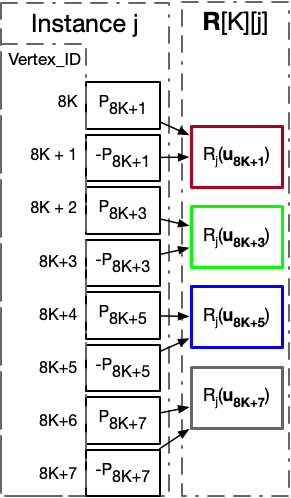
\includegraphics[width=0.7\linewidth, angle=0]{figs/rendering_scheme/texellookup.png}
    \caption{Lookup illustration of the RGBA components of a texel in the texture \textbf{R} indexed by $K$ and $j$. The texel is accessed by the threads that process the 8K, 8K+1, ..., 8K+7 indexed vertices of an instance $j$. The red, blue, green, gray color illustrates the RGBA component of the texel, respectively.}
    \label{fig::texelfetch}
\end{figure}

 %\sout{It is needed so that the first samples of an ODFs do not occupy the RGBA last values of its previous, and it says respect to the 2D texture allocation procedures.} 
 
 The ODF data are accessed in the vertex shader when each glyph instance $j$ is processed. All texels $K = \frac{Vertex\_ID}{8}$ in a column are accessed to get a group of 4 ODF values to displace 8 spherical mesh points. We use the function {\bf texelFetch} to directly access the ODF texture using unnormalized coordinates $(j, \frac{Vertex\_ID}{8})$. The lookup of the ODF component to be used in the thread to deform its respective point in the base geometry in the vertex shader is accessible by analyzing the remainder of Vertex\_ID's division by eight, as illustrated in Fig. \ref{fig::texelfetch}.

%\sout{The columns of the matrix refer to a set of samples of one ODF, which can be accessed directly by the Instance\_ID.}

%\sout{The per-glyph ODF samples are accessed on GPU by its Vertex\_ID. As the elements of the same ODF are contiguous in memory, the RGBA texel sample gives four values of ODF, which are associated to eight points of the mesh. For the same glyph, one texel of index K for a given instance refers to the threads that process vertices that have their respective Vertex\_ID from 8K to 8K+7. The mapping of the texel is illustrated in Fig. \ref{fig::texelfetch}.}

%\sout{Finally, the OpenGL command to perform ODF lookup to deform the spherical mesh for a vertex being processed is texelFetch(\textbf{R}, ivec2( (gl\_VertexID)/8, gl\_InstanceID), 0 ) [(gl\_VertexID\%8)/2]. Note that the use of the bracket notation to access the RGBA component is consistent with the access illustrated in Fig. \ref{fig::texelfetch}.}




%\begin{figure}[ht]
    %\centering
    %\rule{6cm}{3cm}
    %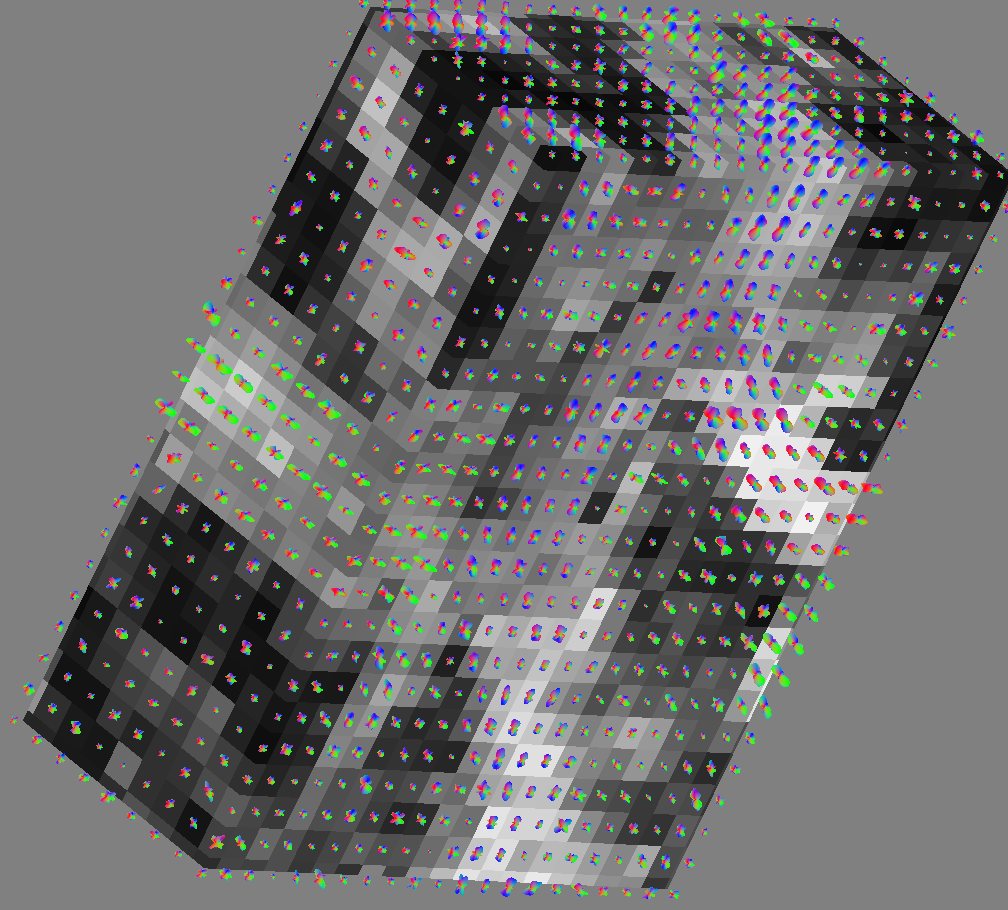
\includegraphics[width=1.00\linewidth, angle=0]{figs/Results/Glyphs_onFAMAP_2.png}
    %\caption{Glyphs integrated into a DW-MRI's fractional anisotropy map. The parallelepiped shows the region where the pyramidal tract (glyphs predominantly blue) crosses the corpus callosum (predominantly red). In the middle of the left face, the predominantly green glyphs corresponds to the region of the superior longitudinal fasciculus. The spherical mesh used corresponds to an 8-th tessellated icosahedron}
    %\label{fig::ex_glyph_FAMAP}
%\end{figure}

%\subsubsection{Glyphs dynamic resolution adjustment}
%\label{ssec::resolution}

%For many small glyphs being rendered, the amount of parameters used may increase the CPU-GPU data traffic to a prohibitive amount of data that penalize the rendering scheme's interactivity. In this section, we show a strategy on how to use different base spherical meshes to be customized by the ODF samples so that it is adaptive and a function of the size that a glyph may occupy on the screen.


%!!Falar de forma generica por aqui?

\section{Experiments, results, and discussion}
\label{sec::results}


We designed an experiment to evaluate the time performance and visual aspects of our proposed ODF glyph rendering integrated into the multimodal rendering environment to assess the enhancement in the conveyance of diffusion data to the superquadrics glyphs, and we also show an experiment that assess the glyph rendering on slices. Time measurements were performed on a Macbook Pro Retina 13' early 2015, with an Intel Core i5 Dual-Core 2.7GHz CPU, 8 GB RAM, and an Intel Iris 6100 GPU with 1536 MB of memory.

The images generated in the experiments were collected as part of the WU-Minn HCP Retest Data by the Connectome Project Consortium \cite{essen2012}. The data used is a DWI and anatomical T1 MRI of an 22-35 years-old healthy woman.

The diffusion data were acquired on a Siemens 3T Skyra scanner. The acquisition is multi-shell 90 diffusion weighting directions for each $b = 1000, 2000$ and $3000 s/mm^2$, and these directions are uniformly distributed in multiple q-space shells, and 6 $b0$ acquisitions for each shell. The data were preprocessed with the HCP diffusion preprocessing pipeline \cite{glasser2013}. The preprocessed acquisition has $145\times 174\times  145$ voxel grid, with sampling space of $1.25x1.25x1.25$mm.

%The diffusion data were acquired on a Siemens 3T Skyra scanner, the acquisition is multi-shell 90 diffusion weighting directions for each $b = 1000, 2000$ and $3000 s/mm^2$, these directions are uniformly distributed in multiple q-space shells, and 6 $b0$ acquisitions for each shell. The data were preprocessed with HCP diffusion preprocessing pipeline, which consisted of b0 intensity normalization across runs, EPI distortion correction, eddy-current-induced distortion correction, motion correction, gradient nonlinearity correction, registration to native structural space, and masking the final data with a brain mask \cite{glasser2013}. The preprocessed acquisition has $145\times 174\times  145$ voxel grid, with sampling space of $1.25x1.25x1.25$mm.

The T1-MRI data were also preprocessed using the HCP minimal preprocessing pipeline \cite{glasser2013}. As its respective DWI, the preprocessed acquisition has $145\times 174\times  145$ voxel grid, with sampling space of $1.25x1.25x1.25$mm.

%The T1-MRI data were also preprocessed using the HCP minimal preprocessing pipeline which consisted of gradient distortion correction, motion correction, registration to Montreal Neurological Institute (MNI) standard space, and intensity normalization \cite{glasser2013}. The data used were smoothed with surface and parcel constrained smoothing of 2mm FWHM. ICA-FIX was included in the preprocessing pipeline, suppressing structured noise and some head motion. As its respective DWI, the preprocessed acquisition has $145\times 174\times  145$ voxel grid, with sampling space of $1.25x1.25x1.25$mm.

%The images used in this study are collected as part of the Healthy Young Adult study in the WU-Minn HCP Retest Data (Essen et al., 2013) by the Human Connectome Project Consortium. The data includes 3T structural and functional MRI for 1,113 adults, 7T resting and task magnetoencephalography (MEG) from 184 subjects, and 3T and 7T diffusion data. Full details of the data can be found in Essen et al. (2012).


%The images used in the experiments were acquired on a Philips Achieva 3T\todo{CONNECTOME HERE!} Scanner on a healthy volunteer (25-year old male). For DWI acquisition, the spin-echo planar diffusion-weighted sequence was applied with 32 diffusion-encoding gradients and a b-value of $1000 s/mm^2$ and one image with a b-value of $0 s/mm^2$. The acquisition parameters were: voxel size=2x2x2mm, no gap, TR=8500 ms, TE=61 ms, flip angle=90, resolution=70x128x128, and FOV=256x256. For T1-weighted spin-echo sequence the acquisition parameters were: voxel size =1x1x1 mm, no gap, TR=7 ms, TE=3.2 ms, flip angle=8, and resolution=180x240x240, and FOV=240x240. All subjects enrolled in the present study signed an informed consent form approved by our university's Ethics Committee.


In the experiment, the imaging method used to obtain the ODFs is the Generalized Q-sampling Imaging \cite{yeh2010}, where the samples are computed and stored in the CPU in a sphere's hemisphere over the $8^{th}$ tessellation order of the icosahedron for all voxels contained in a DWI, giving a total of 321 samples per voxel.







%\todo[inline]{N\~ao revisei daqui para frente ...}
%\subsection{Raw performance}

\subsection{Visual Aspects}



%NÃO FOI POSSÍVEL FAZER COM ORDEM 16 POR FALTA DE MEMÓRIA RAM NO COMPUTADOR, POIS O VOLUME TEM MUITOS VOXELS E OCUPA MAIS MAIS MEMORIA (HARDI) EM RELAÇÃO AO EXPERIMENTO QUE EU TINHA FEITO ANTES.

Fig. \ref{fig::multimodal} shows a coronal slice that contains the centrum semiovale with the fibers of the corpus callosum, coronata radiata. This region presents known crossing fibers and is often used for qualitative analysis. Fig. \ref{fig::multimodal_highres} shows that one can infer about each fiber crossing through the elongated area of the glyph. Note that the glyph resolution is different in \ref{fig::multimodal_lowres} and \ref{fig::multimodal_highres} and it is selected automatically.

In the background, there is the rendering of the anatomical T1-weighted co-registered image. In Fig. \ref{fig::multimodal_highres}, one can see the light-gray areas, that corresponds to the white matter regions, have glyphs rendered on shapes that follows their respective underlying fiber patterns.


\begin{figure}[t]
\centering
\captionsetup[subfloat]{farskip=0pt,nearskip=0pt}
    \subfloat[Coronal slice of T1-MRI co-registered with the DWI. The base geometry is a $2^{th}$ order tessellation of the icosahedron sphere. ]{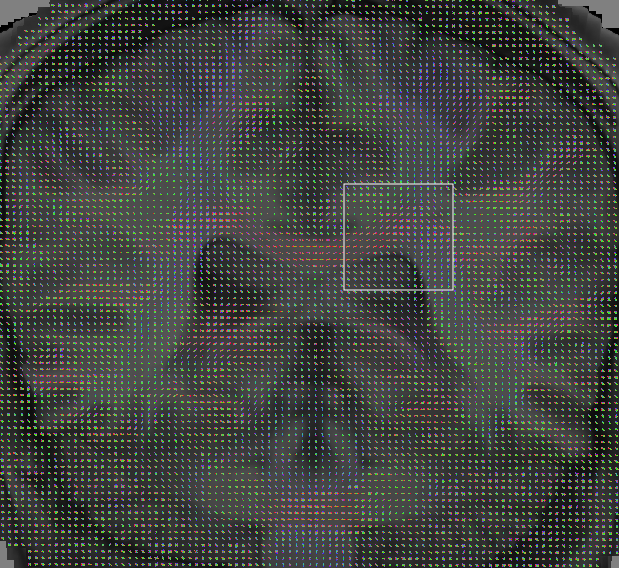
\includegraphics[width=.99\linewidth, angle=0]{figs/Results/Connectomme_Volume/LowResImgHighlighted.png}
    \label{fig::multimodal_lowres}
    }
    \\
    \subfloat[256 glyphs being rendered. The base geometry is a $8^{th}$ order tessellation of the icosahedron sphere.] {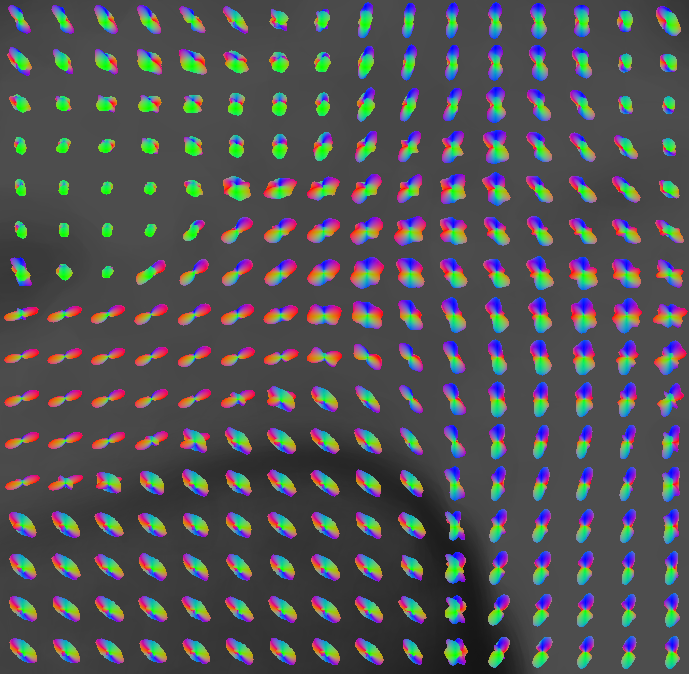
\includegraphics[width=.99\linewidth, angle=0]{figs/Results/Connectomme_Volume/HighResImg.png}
    \label{fig::multimodal_highres}
    }
    \caption{ODF Glyphs integrated into the multimodal visualization for MRI. The image refer to a coronal slice of an anatomical T1 MRI co-registered with the DWI. The glyphs get smoother as occupy more on-screen pixels. The glyphs in the white bounding box in \ref{fig::multimodal_lowres} corresponds to the glyphs in \ref{fig::multimodal_highres}.}
    \label{fig::multimodal}
\end{figure}

Voltoline and Wu \cite{voltoline2021} found evidence that their multimodal rendering with DTI's superquadrics can help on tractography seeding in comparison with color-encoded anisotropy maps. Fig. \ref{fig::multimodal_superquadric} presents the same region of Fig. \ref{fig::multimodal_highres} with DTI's supequadrics. Note that the glyphs have the same problem present on DTI: in fiber crossing, the underlying fiber distribution is not inferable. One can notice by looking at the smoothed rectangular shape in fiber crossing region, where it is not possible to infer about the underlying fiber distribution.

\begin{figure}[ht]
    \centering
    %\rule{6cm}{3cm}
    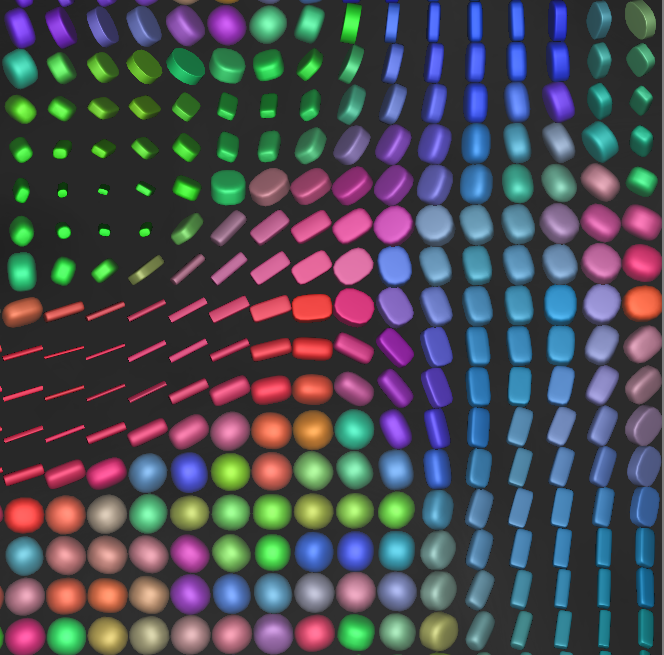
\includegraphics[width=.95\linewidth, angle=0]{figs/Results/Connectomme_Volume/HighResImgSuperquadric.png}
    \caption{Multimodal rendering for DTI's superquadrics. The image corresponds to the region in the white bounding box in Fig. \ref{fig::multimodal_lowres}.}
    \label{fig::multimodal_superquadric}
\end{figure}

\subsection{Performance}


We measured the time performance in FPS of the multimodal rendering for ODF. The number of glyphs is changed through the viewing scaling factor. The greater is the zoom factor, the smaller is the number of glyphs, the higher is each glyph's voxel screen occupancy, increasing their resolution. The output image's resolution is 850x850, and the number of visible glyphs varies between 16 and 6737. The glyphs' resolution varies from the $2^{nd}$ (the lowest level of detail, Figure \ref{fig::multimodal_lowres}) to the $16^{th}$ (the highest level of detail, Figure \ref{fig::multimodal_highres}) tessellation order of the icosahedron. The FPS of the rendering scheme, alongside the number of visible glyphs rendered, the base geometry used, and their respective scaling factors, are listed in Table \ref{tab::glyph_info_experiment}, where we attest that the scheme renders at interactive rates.

\begin{table}[]
\begin{tabular}{|cccc|}
\textbf{FPS} & \textbf{Scaling factor} & \textbf{\# glyphs} & \textbf{\begin{tabular}[c]{@{}c@{}}Tessellation\\ Order\end{tabular}} \\ \hline
32.28 & 86.50 & 12     & 8 \\
33.99 & 58.15 & 20     & 8 \\
34.48 & 38.76 & 42     & 8 \\
33.75 & 25.84 & 90     & 8 \\
33.44 & 17.23 & 210    & 8 \\
33.13 & 11.49 & 420    & 8 \\
32.82 & 7.66  & 930    & 4 \\
34.73 & 5.10  & 2070   & 4 \\
31.19 & 3.40  & 4556   & 4 \\
21.58 & 2.27  & 9931   & 4 \\
17.92 & 1.51  & 13360  & 2 \\
\hline
\end{tabular}
\caption{Glyph Information in image 850 x 850. The number of vertices and triangles of the mesh used is in Table \ref{tab::icosahedron_set}.}
\label{tab::glyph_info_experiment}
\end{table}

\subsection{Slice Rendering}
%\subsubsection{Comparison with Shattuck et al.'s approach}

One may compare our approach with Shattuck et al.'s \cite{shattuck2008}, since both of them are based on polygons, where ODF samples deform a base spherical mesh. In their approach, each ODF was stored as coefficients of base functions on CPU and the glyph shapes were computed on slices. Thus, the computation of each glyph's shape consisted in the computation of the displacement of each vertex in the base spherical mesh using its base function on CPU, and the CPU-GPU data traffic consisted on setting a polygon with its vertex data as a function of the ODF on the base geometry and send the shape's vertex data to GPU and then use commands to delimit a set of primitives to draw.

On our approach, we set the base geometries a priori and store ODF data as samples and showed techniques to select the adequate base geometry, and strategies to handle the CPU-GPU data-traffic bottleneck. To achieve this goal, we showed a way of organizing the ODF and base geometry data to use instance rendering, which was not released at the time Shattuck et al. proposed their work. Furthermore, in the rendering process, we only send to GPU a set of ODF scalar values to displace the base geometry and we deform its points on GPU's threads on each instance. Thus, the per-glyph CPU-GPU data traffic consists $N/2 + (-N/2 \mod{4})$ floats for a base geometry with $N$ vertices, and these values are disposed sequentially, so we can take advantage on GPU's cache. The possibility to decrease the traffic to this amount has been crucial to render these glyphs with fine meshes at interactive rates. Furthermore, the glyphs are rendered with one draw call and the maximum amount of glyphs are limited to the maximum amount of elements allowed on a single texture.

%In order to make a comparison between our and Shattuck et al.'s \cite{shattuck2008} approach when it comes to per-glyph CPU-GPU data traffic, lets consider a generic tessellation order of the icosahedron with N vertices, where each vertex is common to six triangles\footnote{The 12 vertices of the base icosahedron in the mesh are vertices of only five triangles, but for sake of demonstration simplicity, we won't take it into consideration}.

%Considering that Shattuck et al. \cite{shattuck2008} assembled quadrilaterals to form the glyphs surface, which is formed by two triangles, they send to GPU three copies of the same vertex of a point in the glyph's surface to form the glyph. This gives a total of $3\times N$ points sent to GPU, which corresponds to $9\times N$ floats, followed by an individual translation displacement and a drawing command.

%In our approach, the per-glyph data traffic is only related to ODF samples in a half-sphere, which corresponds to  floats, in addition to its respective translation attribute, which is already on GPU. Thus, in our approach, we set the CPU-GPU data traffic to be 5-7\% of the amount of Shattuck et al.'s approach. 

Since our approach is attached to a raycasted DWI volume and a voxel detection algorithm, only the visible voxels are requested to be rendered and it is not restricted to a full slice. Moreover, in the interactive visualization environment, where the user has the possibility of zooming and moving the scene, the voxel detection makes sure that off-screen voxels' ODF coefficients are not sent to GPU and demanded to be processed in the vertex processing stage on GPU's pipeline to be further discarded in rasterization.

%\subsubsection{Derived Applications}

Our scheme can also be applicable to a slice-based glyph rendering. Note that, instead of using the visible voxels set $D$, one can refer the index set to be rendered that refers to a full slice of size $W \times H$. Furthermore, instead of using the translation attributes to place the glyphs in the volume space, one may position the glyph to the center of each block, computed by the subdivision of the scene in rectangles by the dimensions of the slice in dimensions of a slice and scale it accordingly to the dimensions of the block and use instance rendering.

In order to give some performance results of the presented rendering algorithm on 2D-slice rendering, we made the following experiment: the x and y axis is divided in $S$ intervals each ($S = W = H$), giving a grid with $S^2$ equally sized squared regions, which have glyphs rendered in each one of them. Each glyph is scaled to fit in its respective square and placed at its center. The base geometry is fixed, and the translation attributes and the ODF samples matrix in each drawing request is updated and sent to GPU as described in subsection \ref{ssec::glyph_attributes}. We measured the FPS as a function of the amount rendered of glyphs with the $S$ varying until 100. The graphical representation is annotated in Fig. \ref{fig::slice_benchmark} for different base geometries used.

\begin{figure}[ht]
    \centering
    %\rule{6cm}{3cm}
    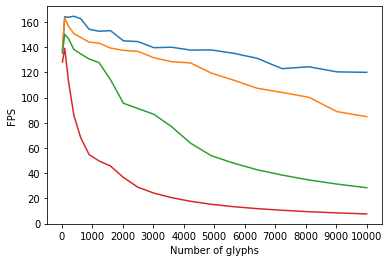
\includegraphics[width=.95\linewidth, angle=0]{figs/Benchmark/benchmark_half_texopt.png}
    \caption{Slice glyph rendering FPS $\times$ number of glyphs being rendered. The blue, orange, green and red curves correspond to a base geometry generated by the $2^{nd}$ $4^{th}$, $8^{th}$ and $16^{th}$ tessellation order of the icosahedron. Their amount of vertices and triangles are in the table \ref{tab::icosahedron_set}.}
    \label{fig::slice_benchmark}
\end{figure}

The results indicate that our scheme gives satisfactory results for interactive usage, and we showed that it is possible to render thousands of glyphs in interactive rates using a $4^{th}$ order tessellation of the icosahedron and hundreds with the $16^{th}$ tessellation order.





 %The ODF data structures setup process in CPU is accelerated by using parallelism.


%\subsection{Time performance}

%In Fig. \ref{fig::benchmark_full} and \ref{fig::benchmark_half} follow the benchmark of the rendering scheme without and with the optimization for symmetrical ODFs. The data structures setup process is accelerated by using CPU parallelism. The computer used was a Macbook Pro Retina 13' early 2015, with an Intel Core i5 Dual-Core 2.7GHz CPU, 8 GB RAM, and an Intel Iris 6100 GPU with 1536 MB of memory.

 
%The computer used was a Macbook Pro Retina 13' early 2015, with an Intel Core i5 Dual-Core 2.7GHz CPU, 8 GB RAM, and an Intel Iris 6100 GPU with 1536 MB of memory.

%The experiment consisted of measuring the FPS as a function of the number of glyphs for the whole rendering process described in section \ref{sec::odf_glyph_rendering} from data taken from a slice. When measuring, all the ODFs samples sent to the GPU are rasterized and drawn for the number of glyphs chosen. The base meshes were the spheres obtained by the $2^{nd}$, $4^{th}$, $8^{th}$, $16^{th}$ tessellation order of the icosahedron, which amount of vertices and triangles are in table \ref{tab::icosahedron_set}. Fig \ref{fig::ex_glyph} exemplifies the glyphs generated by these base geometries for a DWI data.

%  \begin{figure}[ht]
%  \centering
%  \captionsetup[subfloat]{farskip=0pt,nearskip=0pt}
%      \subfloat[$2^{nd}$ order.]{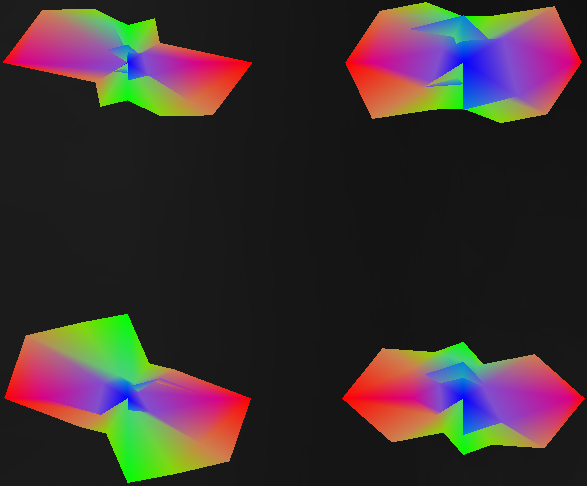
\includegraphics[width=.38\linewidth, angle=0]{figs/Results/Glyphs_2.png}
%      \label{fig::ex_glyph2}
%      }
%     %\hline
%      \subfloat[$4^{th}$ order.]{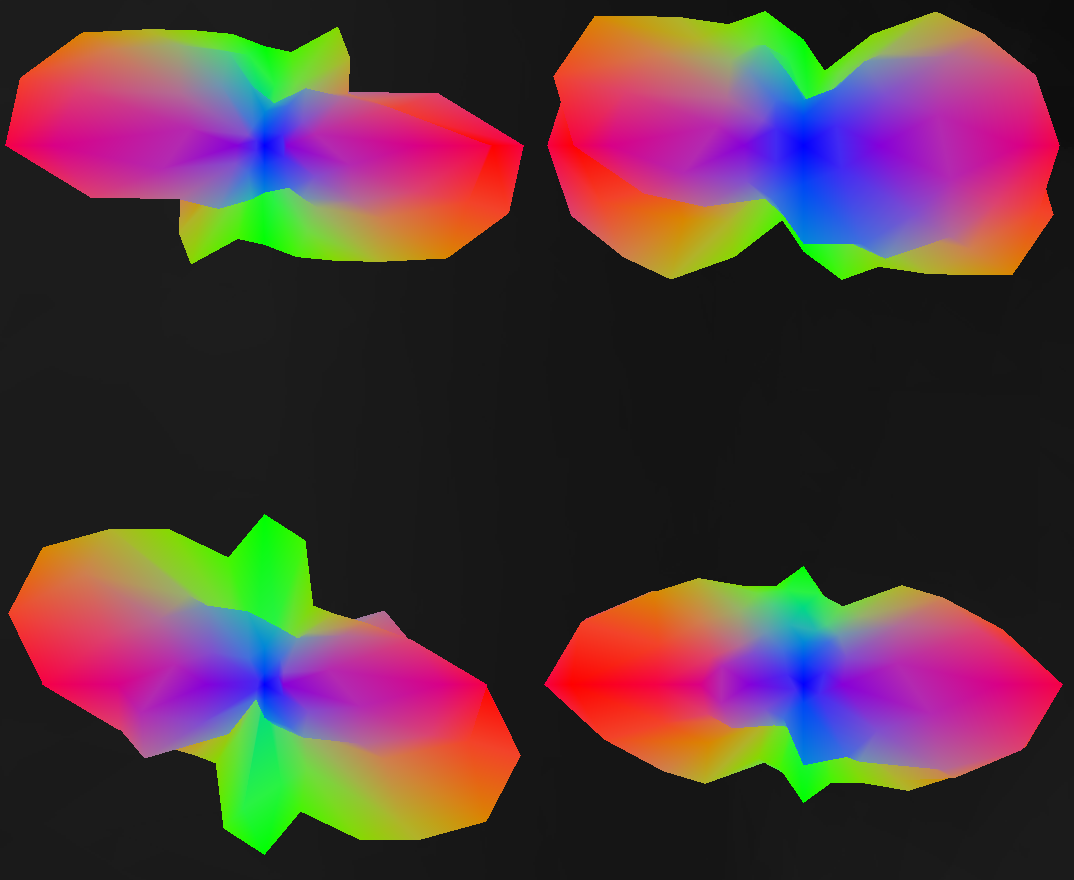
\includegraphics[width=.38\linewidth, angle=0]{figs/Results/Glyphs_4.png}
%      \label{fig::ex_glyph4}
%      }
%      \\
%      \subfloat[$8^{th}$ order.]{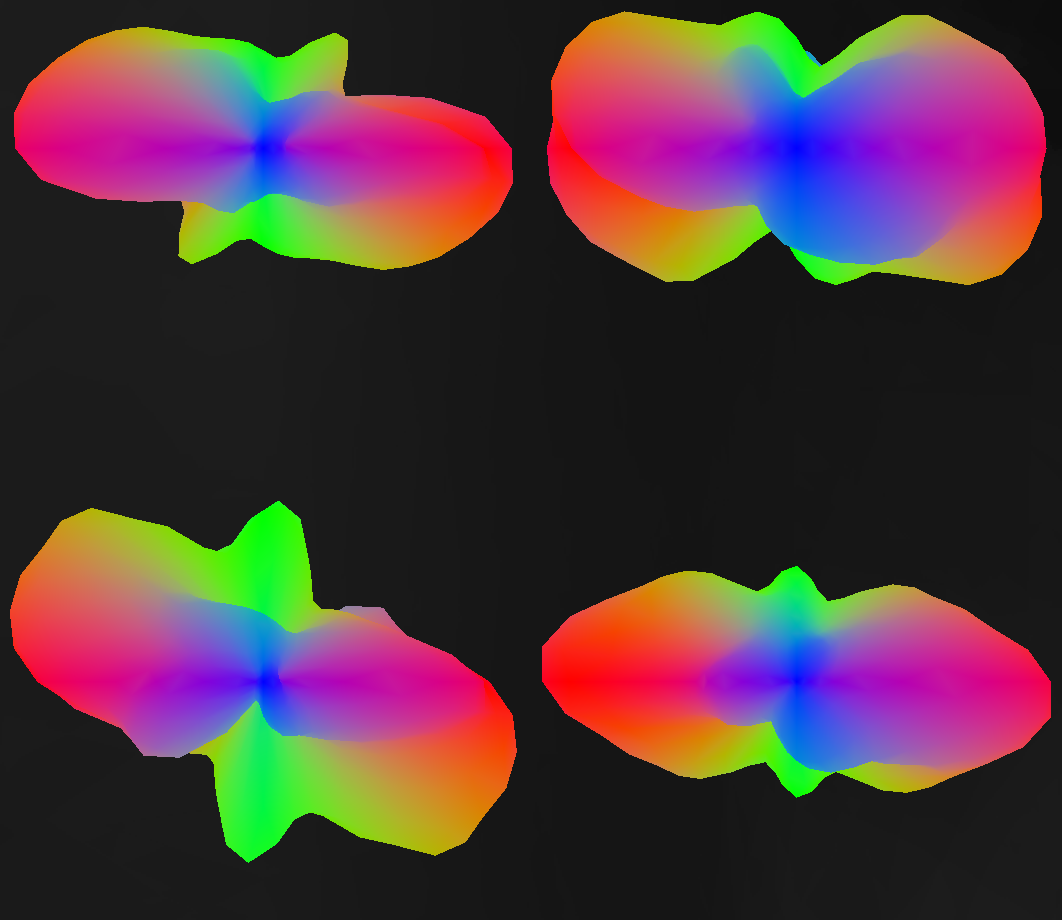
\includegraphics[width=.38\linewidth, angle=0]{figs/Results/glyphs_8.png}
%      \label{fig::ex_glyph8}
%      }
%      %\hline
%      \subfloat[$16^{th}$ order.]{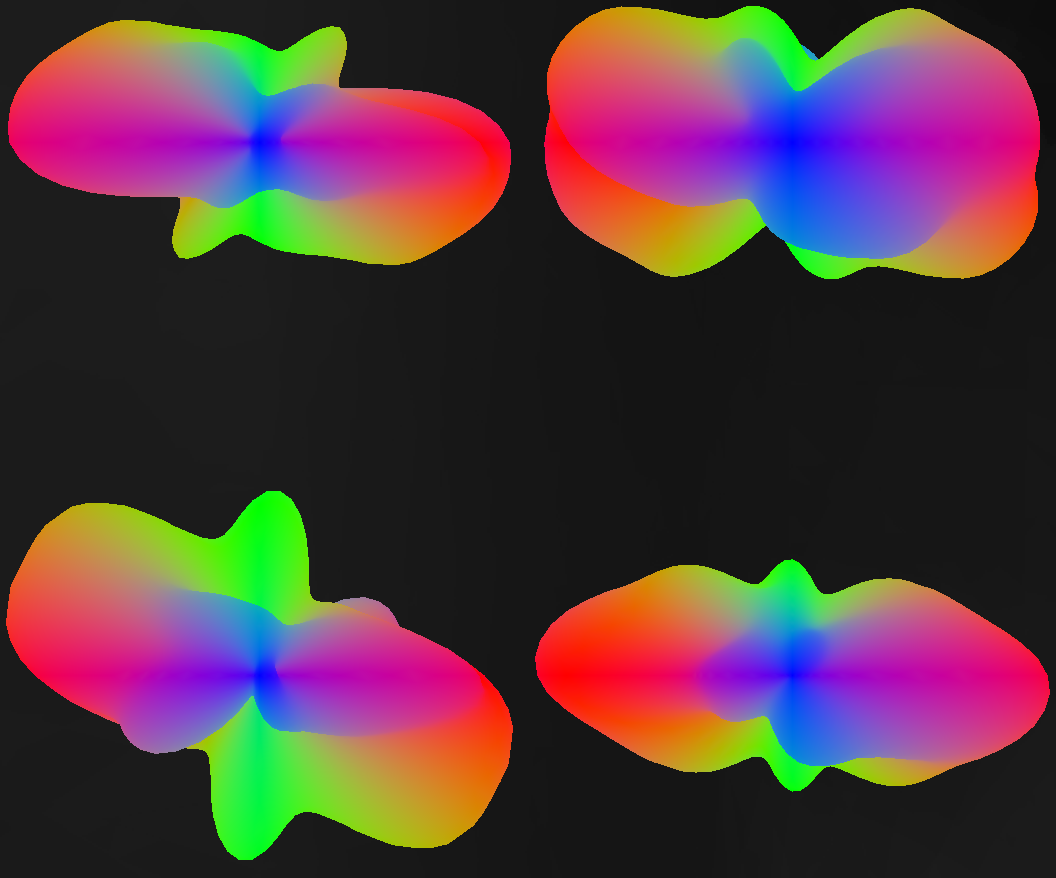
\includegraphics[width=.38\linewidth, angle=0]{figs/Results/glyphs_16.png}
%      \label{fig::ex_glyph16}
%      }
%       \caption{Polygon based HARDI glyphs visualization for different orders of tessellation of an icosahedron. The glyphs refer to the same DWI samples, with 32 gradient directions and b=1000$s/mm^2$ in the region of the corpus callosum in a axial slice. } %!!VER SE ISSO TA CERTO
%      \label{fig::ex_glyph}
%  \end{figure}

%\begin{figure}[ht]
%\centering
%\captionsetup[subfloat]{farskip=0pt,nearskip=0pt}
%    \subfloat[General rendering scheme for ODFs benchmark ]{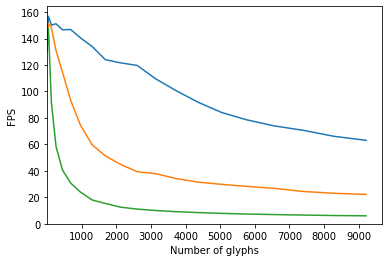
\includegraphics[width=.99\linewidth, angle=0]{figs/Benchmark/benchmark_full.png}
%    \label{fig::benchmark_full}
%    }
%    \\
%    \subfloat[Optimized rendering scheme for symmetrical ODFs benchmark ]{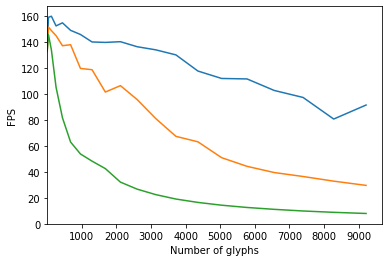
\includegraphics[width=.99\linewidth, angle=0]{figs/Benchmark/benchmark_half.png}
%    \label{fig::benchmark_half}
%    }
%    \\
%     \caption{Glyph rendering FPS $\times$ number of glyphs being rendered. The blue, orange, green and red curves correspond to a spherical mesh  generated by the $2^{nd}$ $4^{th}$, $8^{th}$ and $16^{th}$ order tessellation of the icosahedron. Their amount of vertices and triangles are in the table \ref{tab::icosahedron_set}.} %!!VER SE ISSO TA CERTO
%    \label{fig::benchmark}
%\end{figure}
% \begin{figure}[ht]
%     \centering
%     %\rule{6cm}{3cm}
%     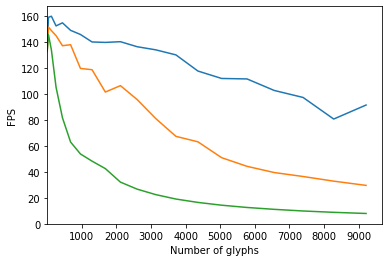
\includegraphics[width=1.00\linewidth, angle=0]{figs/Benchmark/benchmark_half.png}
%     \caption{Glyph rendering FPS $\times$ number of glyphs being rendered. The blue, orange, green and red curves correspond to a spherical mesh  generated by the $2^{nd}$, $4^{th}$, $8^{th}$, and $16^{th}$ order tessellation of the icosahedron. Their amount of vertices and triangles are in the table \ref{tab::icosahedron_set}.
%     }
%     \label{fig::benchmark}
% \end{figure}




%\subsection{Multimodal Rendering}
%\label{ssec::multimodal}

%In this subsection, we describe the implementation of the glyph rendering scheme in a multimodal visualization scheme for DWI, proposed by Voltoline and Wu \cite{voltoline2021}.



%Fig. \ref{fig::ex_glyph_DWI_visualization} show the result of the proposed rendering scheme applied to this environment.

%\begin{figure}[ht]
%    \centering
%    %\rule{6cm}{3cm}
%    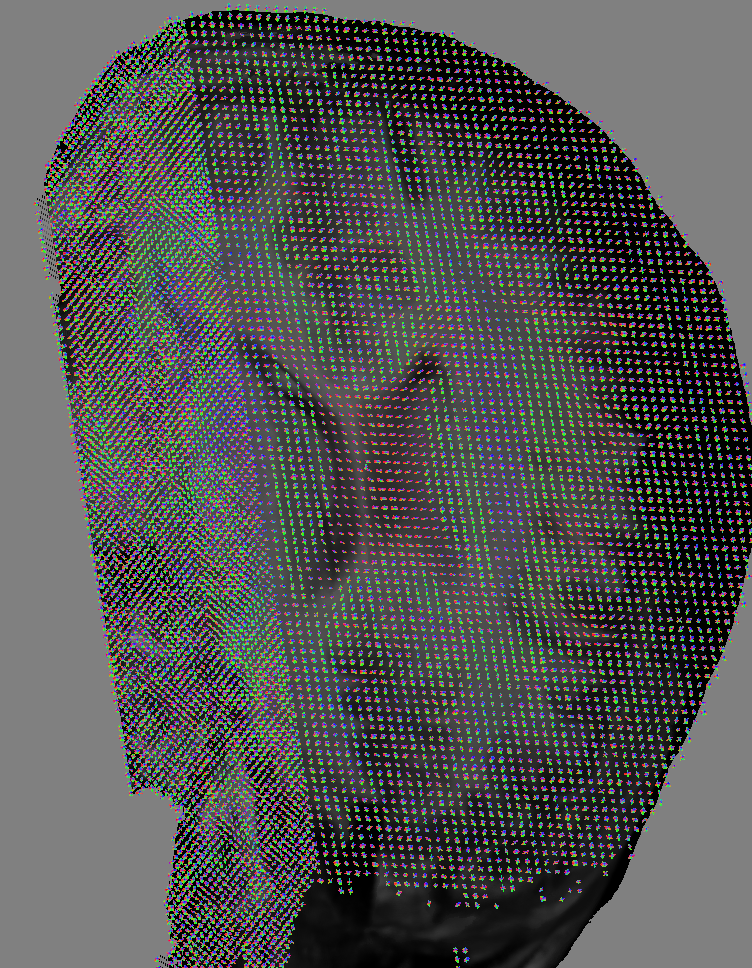
\includegraphics[width=1.00\linewidth, %angle=0]{figs/Results/glyphs_integrated_DWI.pn%g}
%    \caption{Glyphs integrated into a DWI's %visualization scheme. The glyphs are located %in a mid axial region of the brain, cut in the %left side. The spherical mesh used to generate %the glyphs corresponds to an 8-th tessellated %icosahedron. The DWI was acquired with 32 %gradient directions and $b=1000s/mm^2$.
%    }
%    \label{fig::ex_glyph_DWI_visualization}
%\end{figure}



%\subsubsection{Multimodal rendering scheme setup}





% Their respective translation coordinates to its center in the volume space were computed as well, accordingly to Eq. \ref{eq::translation}.

%The multimodaThere is a ray casting-based rendering scheme for MRI/DWI volumes and a algorithm that estimates the on-screen voxels indices and its respective occupancy detection proposed by Voltoline and Wu \cite{voltoline2021}.


%Fig. \ref{fig::vmtk_simplified} shows a simplified flowchart of the rendering scheme, which states the CPU and GPU tasks for visualization. The multimodal visualization is formed by a ray-casted composition of a DWI volume, blended with its respective anatomical T1 MRI co-registered. Additionally, the scheme performs an on-screen voxel detection and estimates its respective size so that only the glyphs of detected voxels are rendered.

%In order to detect the visible voxels and estimate their screen occupancy, in the process of ray casting the volume, there is a GPU-based algorithm that stores the on-screen DWI's voxels coordinates in the on-screen framebuffer. The set of voxel indices and the maximum amount of pixels that render a single voxel ($max_p$) are computed on GPU and transferred to the CPU. The list of detected voxel indices establishes the glyphs to be rendered; the metric $max_p$ defines the mesh's resolution to be used.

%\begin{figure}[ht]
%    \centering
%    %\rule{6cm}{3cm}
%    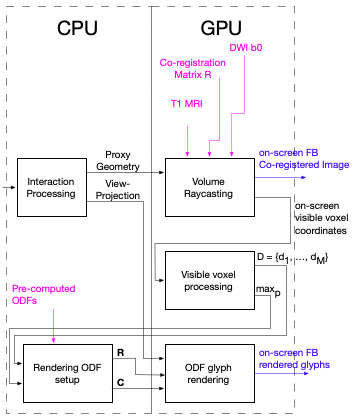
\includegraphics[width=1.0\linewidth, angle=0]{figs/rendering_scheme/fluxograma_glifosVMTK_4.png}
%    \caption{Multimodal rendering for ODF glyphs. The blue color represents the output to be drawn on the framebuffer (FB); the magenta color refers to pre-computed elements. The Volume Raycasting and visible voxel processing stages are proposed by Voltoline and Wu \cite{voltoline2021}. The Rendering ODF setup and ODF glyph rendering stages are described in section \ref{sec::odf_glyph_rendering}.}
%    \label{fig::vmtk_simplified}
%\end{figure}



%returns their respective indexes of the volume, which serves as the basis for the setup of the translation coordinates buffer and ODF data. The setup is made by copying the pre-computed data into the format discussed in the subsection \ref{ssec::datastruct} and sent to GPU. This process to ODF samples is illustrated in Fig. \ref{fig::vmtk_precomputed2GPU}.



%The spherical mesh used is chosen at run time as a function of $max_p$, and in addition to the $16^{th}$ order,  we used the $2^{nd}$, $4^{th}$, and $8^{th}$ order mesh, whose vertices set $\Pi_1$, $\Pi_2$, and $\Pi_3$, satisfy the relation stated in the expression \ref{eq::subset_condition}, as shown in the appendix. The selection criterion is a function of $max_p$, as presented in the subsection \ref{ssec::glyph_resolution}, their respective values $\delta_1$, $\delta_2$, and $\delta_3$ are 225, 3600, and 57600 respectively. Their computation is a function of the number of triangles presented in the table \ref{tab::icosahedron_set}, accordingly to the expression $\delta = (\tau/8)^2$, presented in the subsection \ref{ssec::glyph_resolution}. Fig. \ref{fig::multimodal} illustrates the ODF glyphs visualization comparatively at highest and lowest level of detail.




%The FPS results in the environment as a function of the glyphs amount rendered are presented in Fig. \ref{fig::vmtk_benchmark}.

% \begin{figure}[hb]
%     \centering
%     %\rule{6cm}{3cm}
%     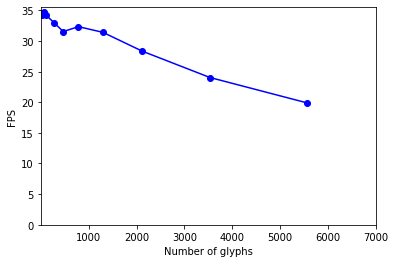
\includegraphics[width=1.0\linewidth, angle=0]{figs/Benchmark/FPS_vmtk_2.png}
%     \caption{ODF Glyph rendering FPS $\times$ number of visible glyphs.}
%     \label{fig::vmtk_benchmark}
% \end{figure}



%\todo[inline]{To assess the fiber orientations locally?}

%\subsection{Discussion}

%The results indicate that our scheme gives satisfactory results for interactive usage. and it is possible to render thousands of glyphs in interactive rates using a $4^{th}$ order tessellation of the icosahedron and hundreds with $16^{th}$ order.

%There is a relevant performance difference in the scheme by taking advantage of the ODF's symmetry. For example, in the 642 vertices spherical mesh, without optimization, the graphic hits 60 FPS with less than 2000 glyphs rendered, while taking advantage of the symmetry of ODFs makes it possible to render 4000, obtaining similar performance.

%One can make a comparison in a scheme where the per-glyph data traffic consists of vertices of triangles. Let us consider a $N$-sized spherical mesh, where each point is a vertex of 6 triangles, which is characteristic of a tessellated icosahedron. The data traffic of our approach per glyph consists of N/2 numbers plus one copy of translate coordinates, and the customization of the glyphs is done per vertex in parallel in the GPU. The information on how to set the triangles is provided once in the initialization process.

%The polygon-based approach proposed by Shattuck et al. \cite{shattuck2008} did not use GPU programming to render glyphs; furthermore, instance rendering was not available when the work was proposed. The glyph customization is done in CPU, where the surface vertices are computed from its basis function and the CPU-GPU data traffic consisted on the set of vertices extracted from the used spherical mesh with some redundant data information so that the graphics API can form the polygons. For a base geometry of $N$ points, the amount of vertices data traffic is higher than $3N$ numbers for each glyph. Hence, our approach's data traffic is less than 1/6 for the same spherical mesh for symmetrical ODF glyphs, which makes the interactivity possible.

%Having shown that our rendering algorithm can draw ODF glyphs in interactive rates, it can be integrated to a multimodal interactive visualization rendering scheme for DWI, where the base mesh resolution and the rendered glyphs amount are demanded in real time, as we show in the experiment described in the subsection \ref{ssec::multimodal}.

%In our approach, that amount of data traffic goes to N/2 floats. Other polygon-based approaches, such as using sending vertices of the glyphs associated to an index buffer, makes the data traffic go to 3N floats plus the size of index buffer and, additionally, regarding translation coordinates, one can choose to send this data as an attribute per vertex and increase the data traffic by 3N floats and do on GPU's threads, or the operation can be done on CPU, which is less efficient than sending once per geometry.

%Shattuck et al. \cite{shattuck2008}  do not discuss the data structures sent to GPU in each drawing request and mention that they did not use GPU programming, so 

%the data traffic to setup a glyph is 6 times the same (x,y,z) coordinate of the modulated point, which translate to 18*N floats. If using triangle fan, where the same vertice can define two triangles, that amount goes to 9*N floats



%Albeit we presented means to decrease CPU-GPU data traffic on this polygon-based approach, it is still much higher than the ray casting approaches. In their work, Peeters et al. \cite{peeters2009} mentions a data-traffic of 15 spherical harmonics coefficients per glyph and obtain smoother results than $3^{rd}$ and $4^{th}$ order tessellation of an icosahedron.


%In contrast, these rendering strategies makes possible to increase the resolution of the sphere.

%In comparison with Peeters et al. \cite{peeters2009}, our approach has more data traffic, but the GPU shaders are much simpler an less intensive computationally than the approach suggested in their work.

%Falar da simplicidade é algo relevante?
%In our approach, the GPU shaders are much simpler than the raycasting approach since it only does a lookup on a texture and per-vertex linear transformations, while ray casting approaches bring are more computationally expensive.

%In MRI visualization tools, one may code a HARDI ODFs in two different ways: samples on a sphere and spherical harmonics coefficients. This rendering scheme is straightforward to be used when the data is coded in samples on a sphere, but approach to store HARDI data can be very memory demanding.







%If the ODFs are stored as coefficients of spherical harmonics, it needs a step of sampling over a spherical mesh.


%Mention comparison with raycasting methods


\section{Conclusions}
\label{sec::conclusions}

In this work, we presented an ODFs glyphs rendering algorithm at interactive rates in a multimodal visualization environment. We used a triangle-based approach for ODFs represented by samples. We suggested strategies to tackle the CPU-GPU data traffic problem in drawing requests.

The rendering algorithm proved to be fast enough to render hundreds and thousands of glyphs at interactive rates and can improve research in the area of HARDI.

%We integrated this rendering scheme to Voltoline and Wu's \cite{voltoline2021} interactive multimodal visualization for DWI, and showed that it can be rendered in interactive rates.

%To our knowledge, this scheme, alongside the ray casting approaches \cite{peeters2009,almsick2011}, are the ones that give the possibility for fast and interactive HARDI data exploration.

For future works, we will investigate the integration in the interactive multimodal rendering environment for diffusion images, how to render triangle-based ODF glyphs efficiently for ODFs represented by a function or algebraic expression.

%We also suggested an optimization procedure to decrease the data computation and CPU-GPU data traffic by half on symmetrical ODFs.






%This scheme can be integrated with other DW-MRI and MRI visualization schemes, and we exemplified the application of it as the integration in our visualization tool for DWI.





%The rendering scheme is not only DWI applicable, but to other areas that use ODFs, represented by its samples.

%It can be a useful tool to render each ODF's glyph on its respective area in the scene.

%\section{Future works}


%\begin{itemize}
%\item provide in-depth a performance comparison between the ray casting approach with the approach suggested in this work;
%\item adapt the scheme by changing the data that customize the glyphs from ODF samples to spherical harmonics basis coefficients and compute its samples in GPU;
%\item investigate strategies to change the spherical mesh as a function of the amount and size of glyphs to be rendered in a drawing request, giving the possibility of decreasing its number of vertices in situations where glyphs are small and/or in high number in the scene.
%\end{itemize}







%\section{Page size}
%Permission to make digital or hard copies of all or part of this work for personal or classroom use is granted without fee provided that copies are not made or distributed for profit or commercial advantage and that copies bear this notice and the full citation on the first page. To copy otherwise, or republish, to post on servers or to redistribute to lists, requires prior specific permission and/or a fee. 

%All material on all pages should fit within a rectangle of 16 x 23.7 cm (6.3"x 9.33"), centered on the page horizontally, beginning 2.5 cm (1") from the top of the page and ending with 3,5 cm (1.4") from the bottom.  The right and left margins should be 2.5 cm (1"). The text should be in two 7.6 cm (3") columns with a 0.8 cm (0.3") gutter. 

%\section{Typeset text}
%\subsection*{Normal or Body Text}
%Please use a 10-point Times Roman font, or other Roman font with serifs, as close as possible in appearance to Times Roman in which these guidelines have been set. The goal is to have a 10-point text, as you see here. Please use sans-serif or non-proportional fonts only for special purposes, such as distinguishing source code text. If Times Roman is not available, try the font named Computer Modern Roman. On a Macintosh, use the font named Times.  Right margins should be justified, not ragged.

%\subsection*{Title and Authors}
%The title (Helvetica 18-point bold), authors' names (Helvetica 10-point) and affiliations (Helvetica 10 point) run across the full width of the page -- one column wide. We also recommend e-mail address (Helvetica 10 point). See the top of this page for three addresses. If only one address is needed, center all address text. For two addresses, use two centered tabs, and so on. For more than three authors, you may have to improvise.\footnote{If necessary, you may place some address information in a footnote, or in a named section at the end of your paper, but margins must remain empty.} 

%\subsection*{First Page Copyright Notice}
%Please include 3.8 cm (1.5") text box with the text shown at the bottom of the left column of the first page with the copyright notice.

%\subsection*{Others Pages}
%Others pages start at the top of the page (margin 2.5 cm) and continue in double-column format.  The two columns on the last even page should be as close to equal length as possible. 

%{\bfseries Total length of a paper is max. 8 pages.}

%Footnotes should be Times New Roman 9-point, and justified to the full width of the column.

%Please, use the standard Journal of WSCG format for references -- that is, a numbered list at the end of the article, ordered alphabetically by first author, and referenced by a name in brackets \cite{con00a}. See the examples of citations at the end of this document. Within this template file, use the style named references for the text of your citation.

%The references are also in 9 pt., but that section (see Section \ref{references}) is ragged right. References should be published materials accessible to the public. Internal technical reports may be cited only if they are easily accessible (i.e. you can give the address to obtain the report within your citation) and may be obtained by any reader. Proprietary information may not be cited. Private communications should be acknowledged, not referenced, e.g. "[Adam, personal communication]").

%\subsection*{Page Numbering, Headers and Footers}
%Do not include headers, footers or page numbers in your submission. These will be added when the publications are assembled.

%\begin{figure}[htb]
%    \centering
%    \rule{6cm}{3cm}
%    \caption{Insert caption to place caption below figure.}
%    \label{fig:box}
%\end{figure}

%\begin{table}[htb]
%	\centering
%	\begin{tabular}{|l|l|l|l|}
%	\hline
%	Graphics & Top & In-between & Bottom \\
%	\hline
%	Tables & End & Last & First \\
%	\hline
%	Figures & Good & Similar & Very well \\
%	\hline
%	\end{tabular}
%	\caption{Table captions should be placed below the table}
%\end{table}

%\section{Figures/Captions}
%Place Tables/Figures/Images in text as close to the reference as possible (see Fig.\ref{fig:box}). It may extend across both columns to a maximum width of 16 cm (6.3"). Captions should be Times New Roman 10-points.  They should be numbered (e.g., "Table 1" or "Figure 2"), please note that the word for Table and Figure are spelled out. Figure's and Table's captions should be centered beneath the image, picture or a table.

%\section{Sections}
%The heading of a section should be in Times New Roman 12-point bold in all-capitals flush left with an additional 6-points of white space above the section head.  Sections and subsequent sub- sections should be numbered and flush left. For a section head and a subsection head together (such as Section 3 and Subsection 3.1), use no additional space above the subsection head.

%\subsection{Subsections}
%The heading of subsections should be in Times New Roman 12-point bold with only the initial letters capitalized. (Note: For subsections and subsubsections, a word like the or a is not capitalized unless it is the first word of the header.)

%\subsubsection{Subsubsections}
%The heading for subsubsections should be in Times New Roman 11-point italic with initial letters capitalized and 6-points of white space above the subsubsection head.

%\section{Acknowledgments}
%Our thanks to ACM SIGCHI and SIGGRAPH for allowing us to modify templates they had developed.

%-------------------------------------------------------------------------
% example of algorithm typesetting
% to allow this, uncomment line 
% \RequirePackage[noend]{myalgorithm}
% in the wscg.sty file
% and download that package from Gabriel Zachmann's page http://zach.in.tu-clausthal.de/latex/
%
%
%\begin{algorithm}
%\hrule
%  \centering
%\begin{algorithmic}
%    \STMT $d_{l,r} = f_B(P_1), f_B(P_n)$
%    \WHILE{ $|d_l| > \epsilon $ and $|d_r| > \epsilon $ and $l<r$}
%        \STMT $d_x = f_B(P_x)$
%        \IF{ $d_x < 0$ }
%            \STMT $l, r = x, r$
%        \ELSE
%            \STMT $l, r = l, x$
%        \ENDIF
%    \ENDWHILE
%\end{algorithmic}
%\hrule
%\caption{Example of some pseudo-code}
%\label{fg:code}
%\end{algorithm}

%\section{Appendix}
%\subsection{Two-powered order of tessellated icosahedron meshes as base geometries}
%\label{ssec::ico_example}

%In this section, we show an application on how to alternate meshes of spherical meshes on ODF's sampled over a two-powered order icosahedron's tessellation. This mesh is symmetrical and presents the following property: for $k < n$, the vertices of the $2^{k}$ order tessellated icosahedron is a subset of $2^{n}$.

%The sphere obtained by the tessellation of the icosahedron is a set of spherical meshes often used by the HARDI community. Tuch \cite{TuchQBall2004} and Yeh et al., \cite{yeh2010} in their proposed diffusion imaging methods for HARDI works, use this mesh category in their experiments to show the reconstruction of their respective ODFs. Descoteaux et al. \cite{descoteaux2007} use this category of mesh to project an ODF represented by base functions to compute its underlying fiber configuration. 

%This property can be corroborated by the fact that tessellation of order $2^k$ consists of a subdivision of each triangle of the $2^{k-1}$ tessellation in four. These four triangles vertices' are formed by six points: three of them are the same of the base triangle from $2^{k-1}$-th order, and the other three are derived from these points as they are each pair's projection of the median points onto the sphere as illustrated in Fig. \ref{fig::subdivision_icosahedron}. Table \ref{tab::icosahedron_set} shows the number of vertices and triangles of each tessellation order.

%\begin{figure}[htb]
%    \centering
%    %\rule{6cm}{3cm}
%    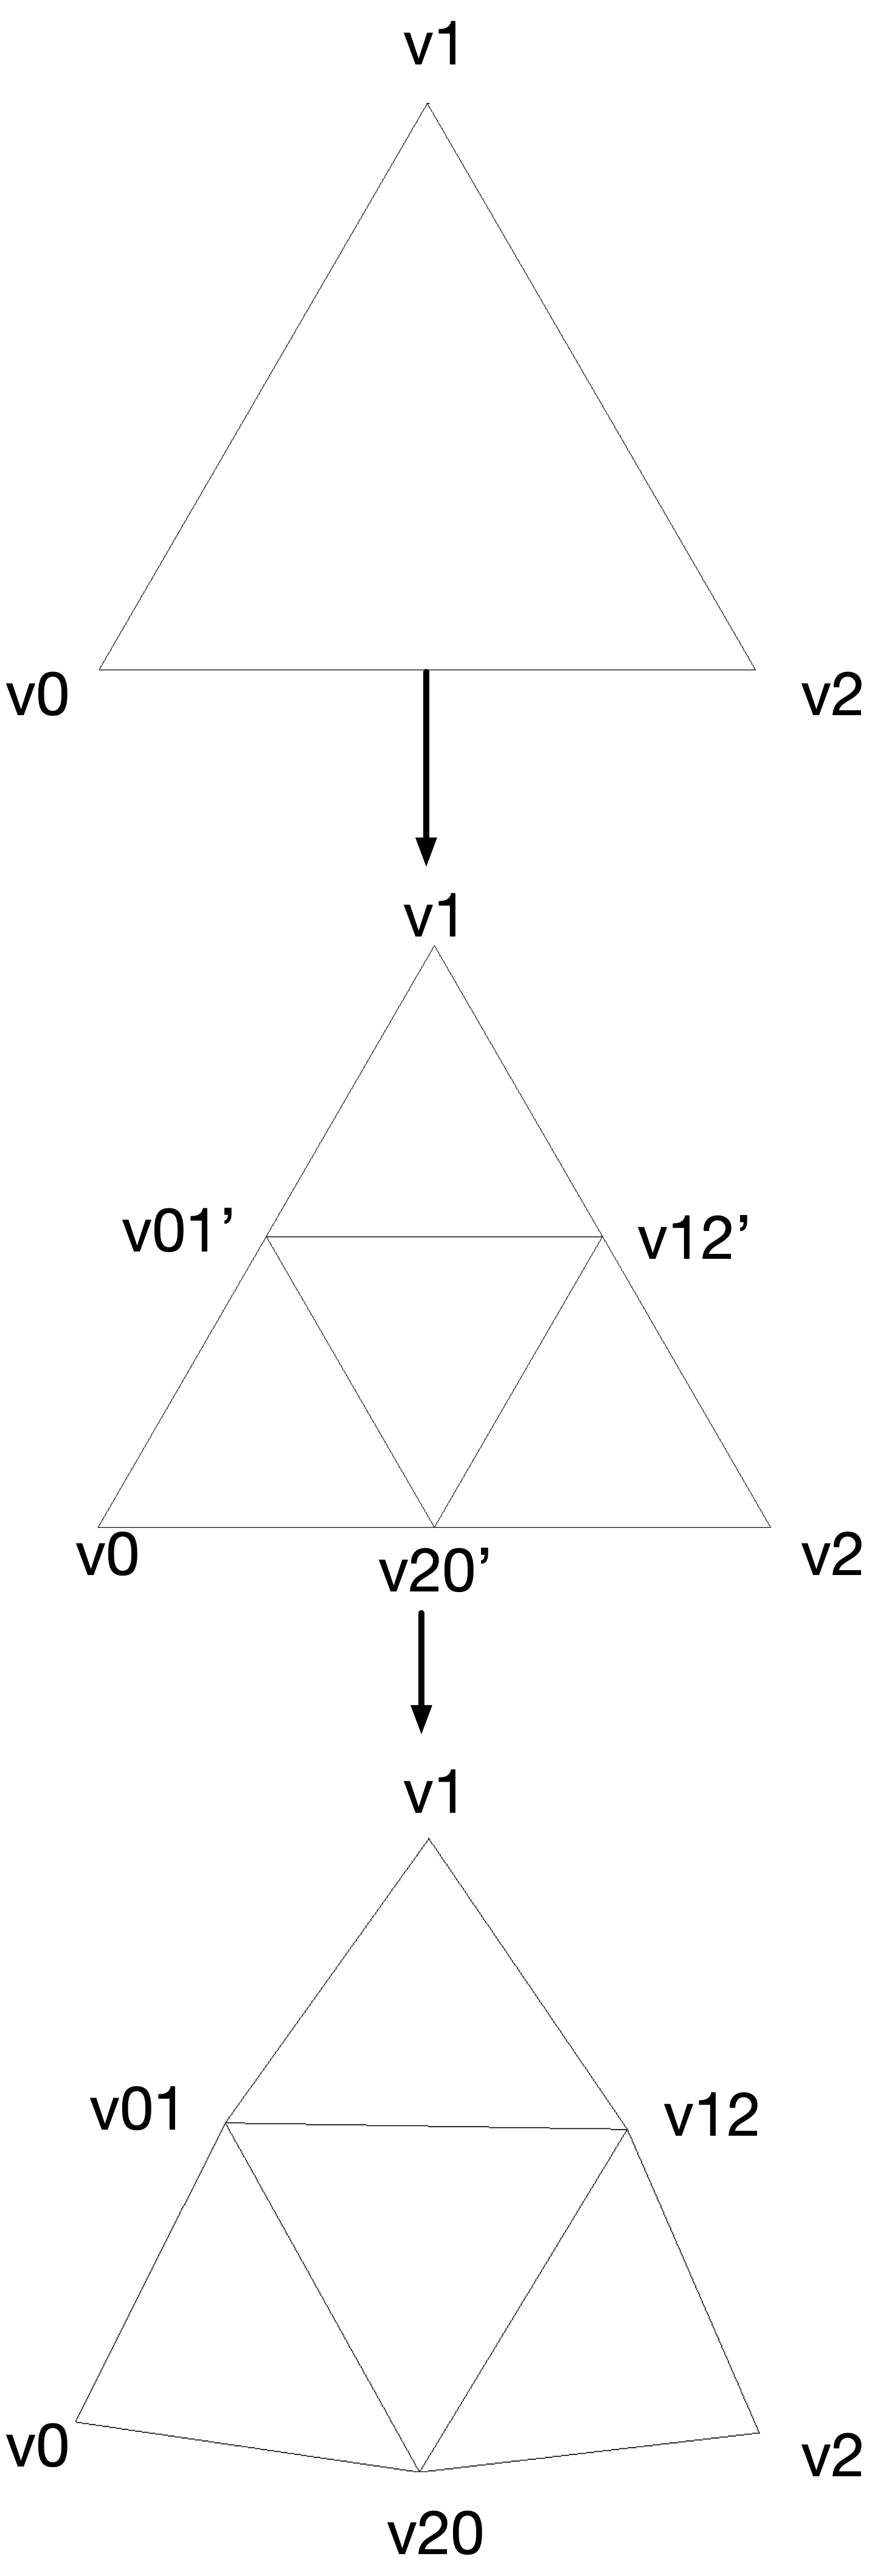
\includegraphics[width=.45\linewidth, angle=0]{figs/icosahedron_example/ico_subdivision_V.png}
%    \caption{Triangle subdivision to form a $2^k$-th order of tessellation of the icosahedron from a $2^{k-1}$-th order. The triangle formed by v0, v1, and v2 is subdivided into four triangles, where the median points v01', v12'and v20' are computed, and their projections on the unit sphere v01, v12, and v20 are added into the vertices set.
%    }
%    \label{fig::subdivision_icosahedron}
%\end{figure}

%Thus, assigning $\Pi$ to be the vertices set of the $2^k$-th order of tessellation of the icosahedron and $\Pi_1$, $\Pi_2$, ..., $\Pi_{k-1}$ to be the $2^{1}$-th, $2^{2}$-th, ..., $2^{k-1}$-th order, respectively, we obtain a set of meshes that satisfy the properties described in the expression \ref{eq::subset_condition}. In practice, we recommend $k$ to be equal to 3 or 4, which requires 321 and 1281 ODF samples per voxel. Values of k above that may incur in a prohibitive amount of memory for ODF samples in a DWI.

%In this section, we are going to consider $\Pi$ as the points of the spherical mesh generated by the $16^{th}$ tessellation order of the icosahedron, which gives $V_N = 2562$ points. Thus, $\Pi_1$, $\Pi_2$ and $\Pi_3$ are the vertices set of the $2^{nd}$, $4^{th}$ and $8^{th}$ order of the tessellated icosahedron, respectively. They 

%$10(2^k+1)(2^k-1)+12$

%Let the set $\Pi_{16} = \{P_1, P_2, ..., P_{2562}\}$ to be correspondent to the $16^{th}$ tessellated icosahedron. Then, we suggest that the data is organized in such a way that its respective subsets $\Pi_{2^k}$, $(k<4)$ is $\{P_1, P_2, ..., P_{V_{2^k}}\}$.

%It means that the first 12 vertices of $\Pi_{16}$ corresponds to the icosahedron's vertices, the first 42 vertices correspond to the $2^{nd}$ order tessellation, the 162 first vertices corresponds to the vertices of the $4^{th}$ tesselation, and the 642 first elements are the points of the $8^{th}$.

%It means $\Pi_1 = \{P_1, P_2, ..., P_{12}\}$ is the vertices set of the icosahedron; $\Pi_2 = \{P_1, P_2, ..., P_{42}\}$, the vertices of the $2^{nd}$ order of the tessellated icosahedron; $\Pi_4 = \{P_1, P_2, ..., P_{162}\}$, the vertices of the $4^{th}$ order and $\Pi_8 = \{P_1, P_2, ..., P_{642}\}$, the $8^{th}$ tessellation order.

%Organizing the vertices lists eases the ODF-related CPU-GPU data traffic. When the glyph is derivated for a $2^k$ order of the tesselation of the icosahedron, the data traffic consists of the first $V_{2^k}$ ODF samples in CPU.

%We suggest that the vertices set of the $16^{th}$ order of the tessellation of the icosahedron is downloaded in the GPU, as well as the index buffers of each order of the icosahedron that are a subset as well.

%Whenever the resolution of the mesh changes, the additional processes that occurs consists on changing the active index buffer to the requested tessellation and the modification on the amount of elements that set $\bm{\Psi}$ or $\bm{\Psi^h}$.




%-------------------------------------------------------------------------

\printbibliography
%\begin{thebibliography}{99}
%\label{references}
%\label{references}
%\bibitem[And01a]{and01a} Anderson, R.E. Social %impacts of computing: Codes of professional %ethics. Social Science, pp.453-469, 2001.
%\bibitem[Con00a]{con00a} Conger., S., and Loch, %K.D. (eds.). Ethics and computer use. Com.of ACM %38, No.12, 2000.
%\bibitem[Con00b]{con00b} Mackay, W.E. Ethics, lies %and videotape, in Conf.proc. CHI'00, Denver CO, %ACM Press, pp.138-145, 2000.
%\bibitem[Jou01a]{jou01a} Journal of WSCG \& WSCG %templates: http://wscg.zcu.cz/jwscg/template.doc %(MSWord)
%http://wscg.zcu.cz/jwscg/template.pdf (PDF)
%\end{thebibliography}
%{\bfseries


%Last page should be fully used by text, figures etc. Do not leave empty space, please. 
%Do not lock the PDF -- additional text and info will be inserted, i.e. ISSN/ISBN etc. 
%}
\end{document}